
\documentclass[a0,landscape]{a0poster}

\usepackage{multicol} %
\columnsep=100pt 
\columnseprule=3pt 

\usepackage{listings}
\usepackage[usenames,dvipsnames]{color}

\usepackage{times} % Use the times font

\usepackage{graphicx} 
\graphicspath{{figures/}}
\usepackage{booktabs} % Top and bottom rules for table
\usepackage[font=small, labelfont=bf]{caption} % Required for specifying captions to tables and figures
\usepackage{amsfonts, amsmath, amsthm, amssymb} % For math fonts, symbols and environments

\def\graphspacing{\vspace{.5cm}}
\newcommand{\highlight}[1]{{\color{Fuchsia} \textit{#1}}}
\newcommand{\capcolor}[1]{{\color{Black} #1}}
\newcommand{\var}[1]{{\small \textit{#1}}}

% define my own color
\usepackage{xcolor}
\definecolor{comment}{RGB}{120,120,120}
\definecolor{codenumber}{RGB}{100,100,100}
\definecolor{shade}{RGB}{240,240,240}

% enable inserting codes
\usepackage{listings}

\lstset{
  language={Eiffel},
  commentstyle=\color{comment},
  basicstyle=\footnotesize\ttfamily,
  numbers=left,
  numberstyle=\scriptsize\color{codenumber},
  frame=single,		% add the frame
  breaklines=true,	% sets automatic line breaking
 % texcsstyle=*\color{red},
 % identifierstyle=\color{magenta},
  extendedchars,
  escapeinside=``,	% used for escaping
  tabsize=2
}

\begin{document}

%%%%%%%%%%%%%%%%%%%%%%%%%%%%%%%%%%%%%%%%%%%%%%%%%%%%%%%%%%%%%%%%%%%%%%%%%%%%%%%%%%%%%%%%%%%%%%%%%%
%%%%%%%%%%%%%%%%%%%%%%%%%%%%%%%%%%%%% Header %%%%%%%%%%%%%%%%%%%%%%%%%%%%%%%%%%%%%%%%%%%%%%%%%%%%%
%%%%%%%%%%%%%%%%%%%%%%%%%%%%%%%%%%%%%%%%%%%%%%%%%%%%%%%%%%%%%%%%%%%%%%%%%%%%%%%%%%%%%%%%%%%%%%%%%%
\begin{minipage}[b]{0.2\linewidth}
\centering

\includegraphics[width=.75\linewidth]{logos/yorku.png}  
\end{minipage}
%
\begin{minipage}[b]{0.6\linewidth}
\centering
\veryHuge \color{Blue} \textbf{Building an Automated Verifier for a Procedural Programming Language by Applying Propositional and Predicate Logic} \color{Black}  \\ [1cm]
\huge \textbf{Chen-Wei Wang, Xiang Chen} \\ 
\huge Lassonde School of Engineering, York University \\
\LARGE \texttt{\{~jackie@eecs.yorku.ca, xiang2@my.yorku.ca~\}}
\end{minipage}
%
\begin{minipage}[b]{0.2\linewidth}
\centering

\includegraphics[width=.45\linewidth]{logos/lassonde.jpeg}
\end{minipage}

\vspace{1cm} 

\begin{multicols}{4} 
	
	\normalsize
	
% \large

%%%%%%%%%%%%%%%%%%%%%%%%%%%%%%%%%%%%%%%%%%%%%%%%%%%%%%%%%%%%%%%%%%%%%%%%%%%%%%%%%%%%%%%%%%%%%%%%%%
%%%%%%%%%%%%%%%%%%%%%%%%%%%%%%%%%%%%% Abstract %%%%%%%%%%%%%%%%%%%%%%%%%%%%%%%%%%%%%%%%%%%%%%%%%%%
%%%%%%%%%%%%%%%%%%%%%%%%%%%%%%%%%%%%%%%%%%%%%%%%%%%%%%%%%%%%%%%%%%%%%%%%%%%%%%%%%%%%%%%%%%%%%%%%%%
{\color{Blue} % Navy color for the abstract

\begin{abstract}
\noindent
\begin{itemize}
\item The teaching of logic and software engineering courses has always been a challenge since the lacking of an efficient automated tool.
\item We present an automated verifier: 
\begin{itemize}
\item to designing a language, more suitable for the purpose of modeling, which uses an SMT solver (i.e., Z3) as its backend tool.
\item to verifying if a valid propositional or predicate formula is a tautology, and provide a counterexample otherwise.
\item to automatically transforming the routine of a procedural programming language into a number of Hoare Triple.
\item to proving if the specific Hoare Triple is a tautology by systematically calculating the weakest precondition of every routine, given its implementation and postcondition.
\end{itemize}

\end{itemize}

\end{abstract}}

%%%%%%%%%%%%%%%%%%%%%%%%%%%%%%%%%%%%%%%%%%%%%%%%%%%%%%%%%%%%%%%%%%%%%%%%%%%%%%%%%%%%%%%%%%%%%%%%%%
%%%%%%%%%%%%%%%%%%%%%%%%%%%%%%%%%%%%% Background %%%%%%%%%%%%%%%%%%%%%%%%%%%%%%%%%%%%%%%%%%%%%%%%%
%%%%%%%%%%%%%%%%%%%%%%%%%%%%%%%%%%%%%%%%%%%%%%%%%%%%%%%%%%%%%%%%%%%%%%%%%%%%%%%%%%%%%%%%%%%%%%%%%%

{\color{Blue} \subsection*{Background}}

\begin{itemize}
	
\item \highlight{Tautology}~  means a valid (i.e., without any syntax of type errors) formula holds for every interpretation.
\item \highlight{Hoare Triple: $\{Q\} S \{R\}$} is the center feature of the Hoare logic, which is proposed in 1969 by the British computer scientist and logician Tony Hoare, and subsequently refined by Hoare and other researchers. Hoare Triple is a boolean predicate that either can be proved of disproved for verifying the correctness of a computer program.
\item \highlight{Weakest Precondition (wp)} can be used for proving the Hoare Triple. $\{Q\} S \{R\}  \equiv Q \Rightarrow wp(S, R)$

\end{itemize}

%%%%%%%%%%%%%%%%%%%%%%%%%%%%%%%%%%%%%%%%%%%%%%%%%%%%%%%%%%%%%%%%%%%%%%%%%%%%%%%%%%%%%%%%%%%%%%%%%%
%%%%%%%%%%%%%%%%%%%%%%%%%%%%%%%%%%%%% Motivation %%%%%%%%%%%%%%%%%%%%%%%%%%%%%%%%%%%%%%%%%%%%%%%%%
%%%%%%%%%%%%%%%%%%%%%%%%%%%%%%%%%%%%%%%%%%%%%%%%%%%%%%%%%%%%%%%%%%%%%%%%%%%%%%%%%%%%%%%%%%%%%%%%%%

{\color{Blue} \subsection*{Motivation}}

\begin{itemize}
\item An efficient tool for the teaching of logic and software engineering courses is necessary. However, most of the available tool are not designed for teaching. 
\item The input language for an SMT solver (e.g., Z3) may not be so user-friendly.
\end{itemize}

%%%%%%%%%%%%%%%%%%%%%%%%%%%%%%%%%%%%%%%%%%%%%%%%%%%%%%%%%%%%%%%%%%%%%%%%%%%%%%%%%%%%%%%%%%%%%%%%%%
%%%%%%%%%%%%%%%%%%%%%%%%%%%%%%%%%%%% Contributions %%%%%%%%%%%%%%%%%%%%%%%%%%%%%%%%%%%%%%%%%%%%%%%
%%%%%%%%%%%%%%%%%%%%%%%%%%%%%%%%%%%%%%%%%%%%%%%%%%%%%%%%%%%%%%%%%%%%%%%%%%%%%%%%%%%%%%%%%%%%%%%%%%

{ \color{BrickRed}
\subsection*{Contributions}

\begin{enumerate}
\item An automated verifier for propositional and predicate formula.
\item An automated verifier for program verification, including the steps of :
\begin{enumerate}
\item transforming the program routine into a number of Hoare Triple
\item automatically calculating the weakest precondition
\item proving of disproving the Hoare Triple by using the calculated weakest precondition
\end{enumerate}
\item Providing counterexamples if the formula or Hoare Triple is not tautology.
\end{enumerate}
}

%%%%%%%%%%%%%%%%%%%%%%%%%%%%%%%%%%%%%%%%%%%%%%%%%%%%%%%%%%%%%%%%%%%%%%%%%%%%%%%%%%%%%%%%%%%%%%%%%%
%%%%%%%%%%%%%%%%%%%%%%%%%%%%%%%%%%%%% Methodology %%%%%%%%%%%%%%%%%%%%%%%%%%%%%%%%%%%%%%%%%%%%%%%%
%%%%%%%%%%%%%%%%%%%%%%%%%%%%%%%%%%%%%%%%%%%%%%%%%%%%%%%%%%%%%%%%%%%%%%%%%%%%%%%%%%%%%%%%%%%%%%%%%%

{\color{Blue} \subsection*{Methodology}}

\begin{center}\graphspacing
\centering
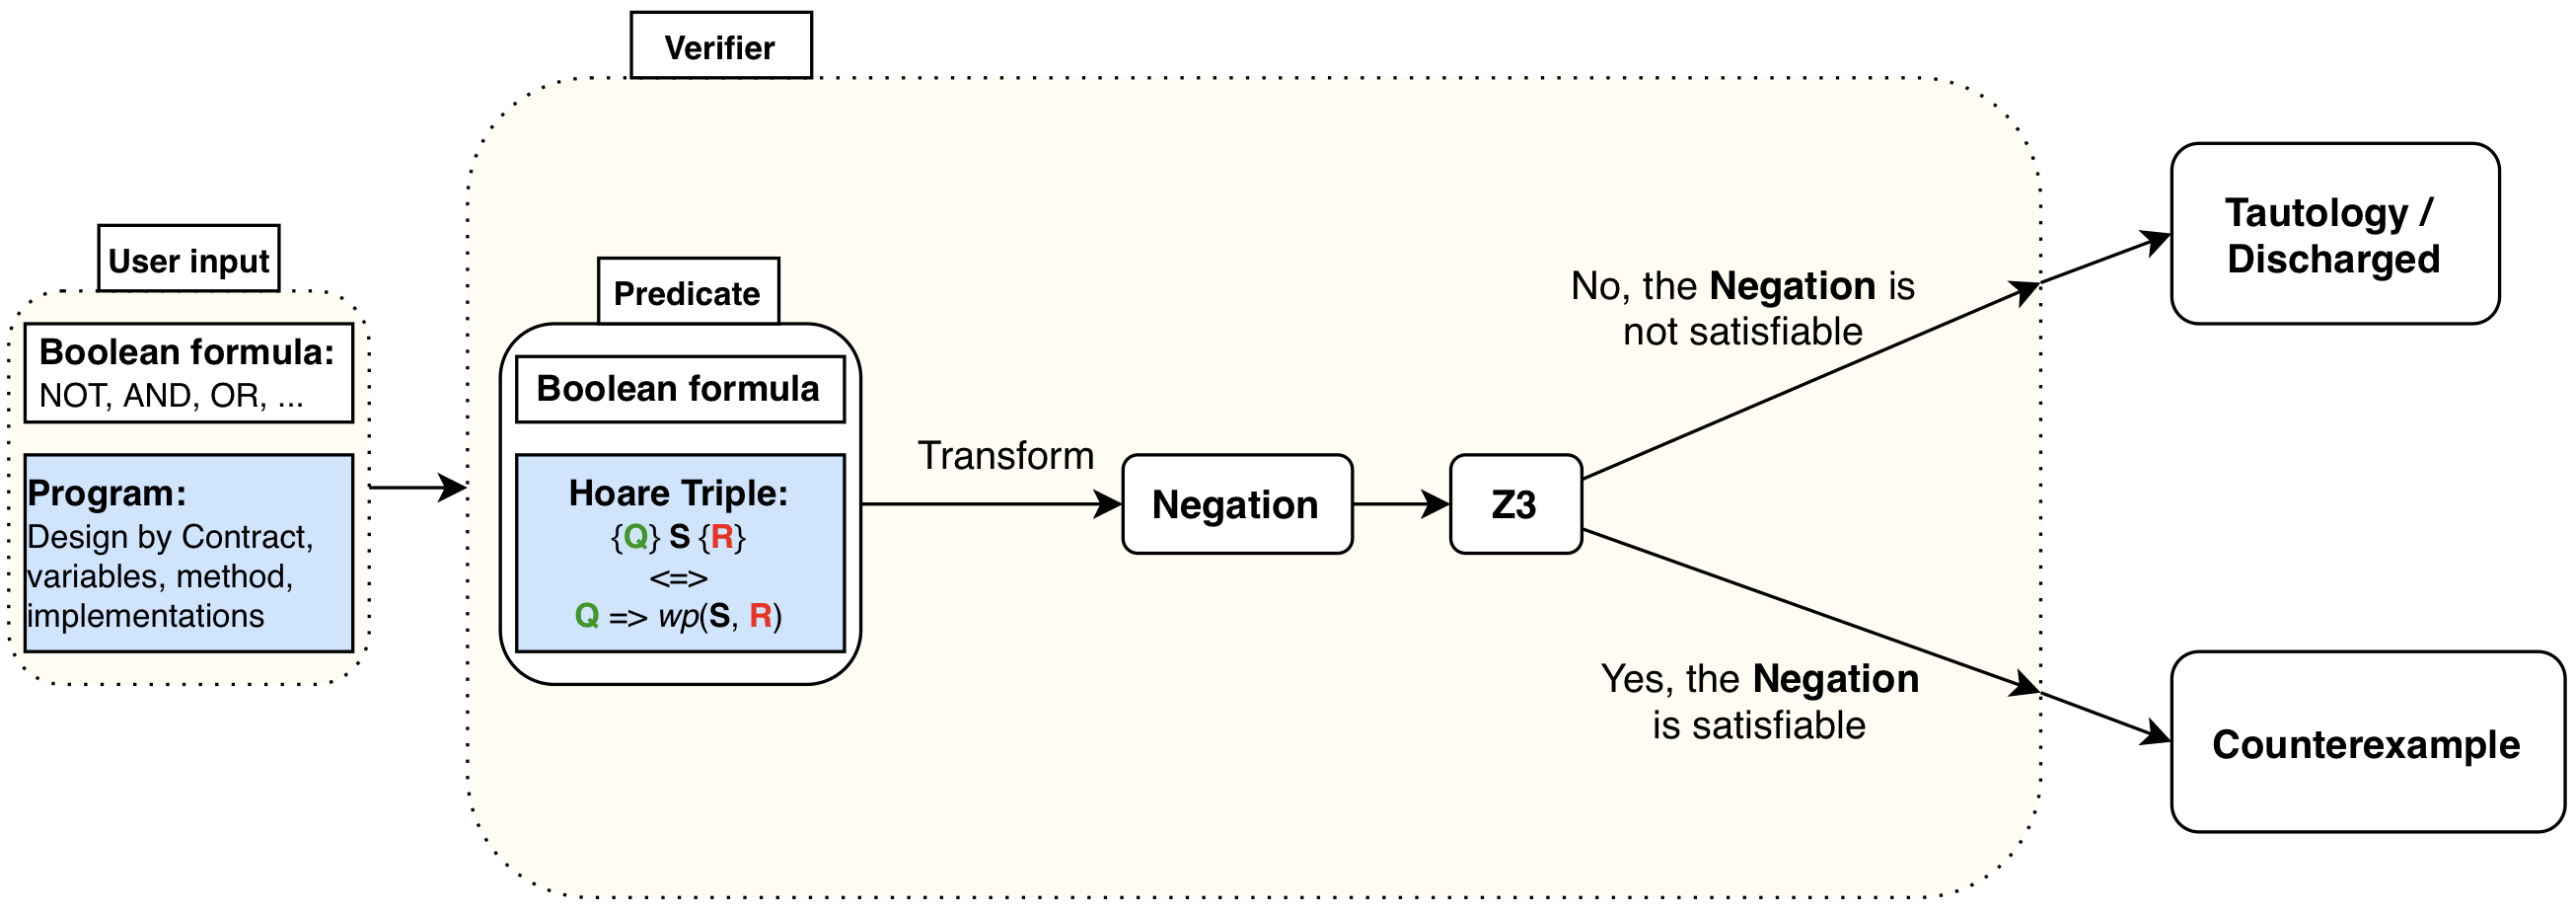
\includegraphics[width=\linewidth]{figures/myTool-extension.jpg}
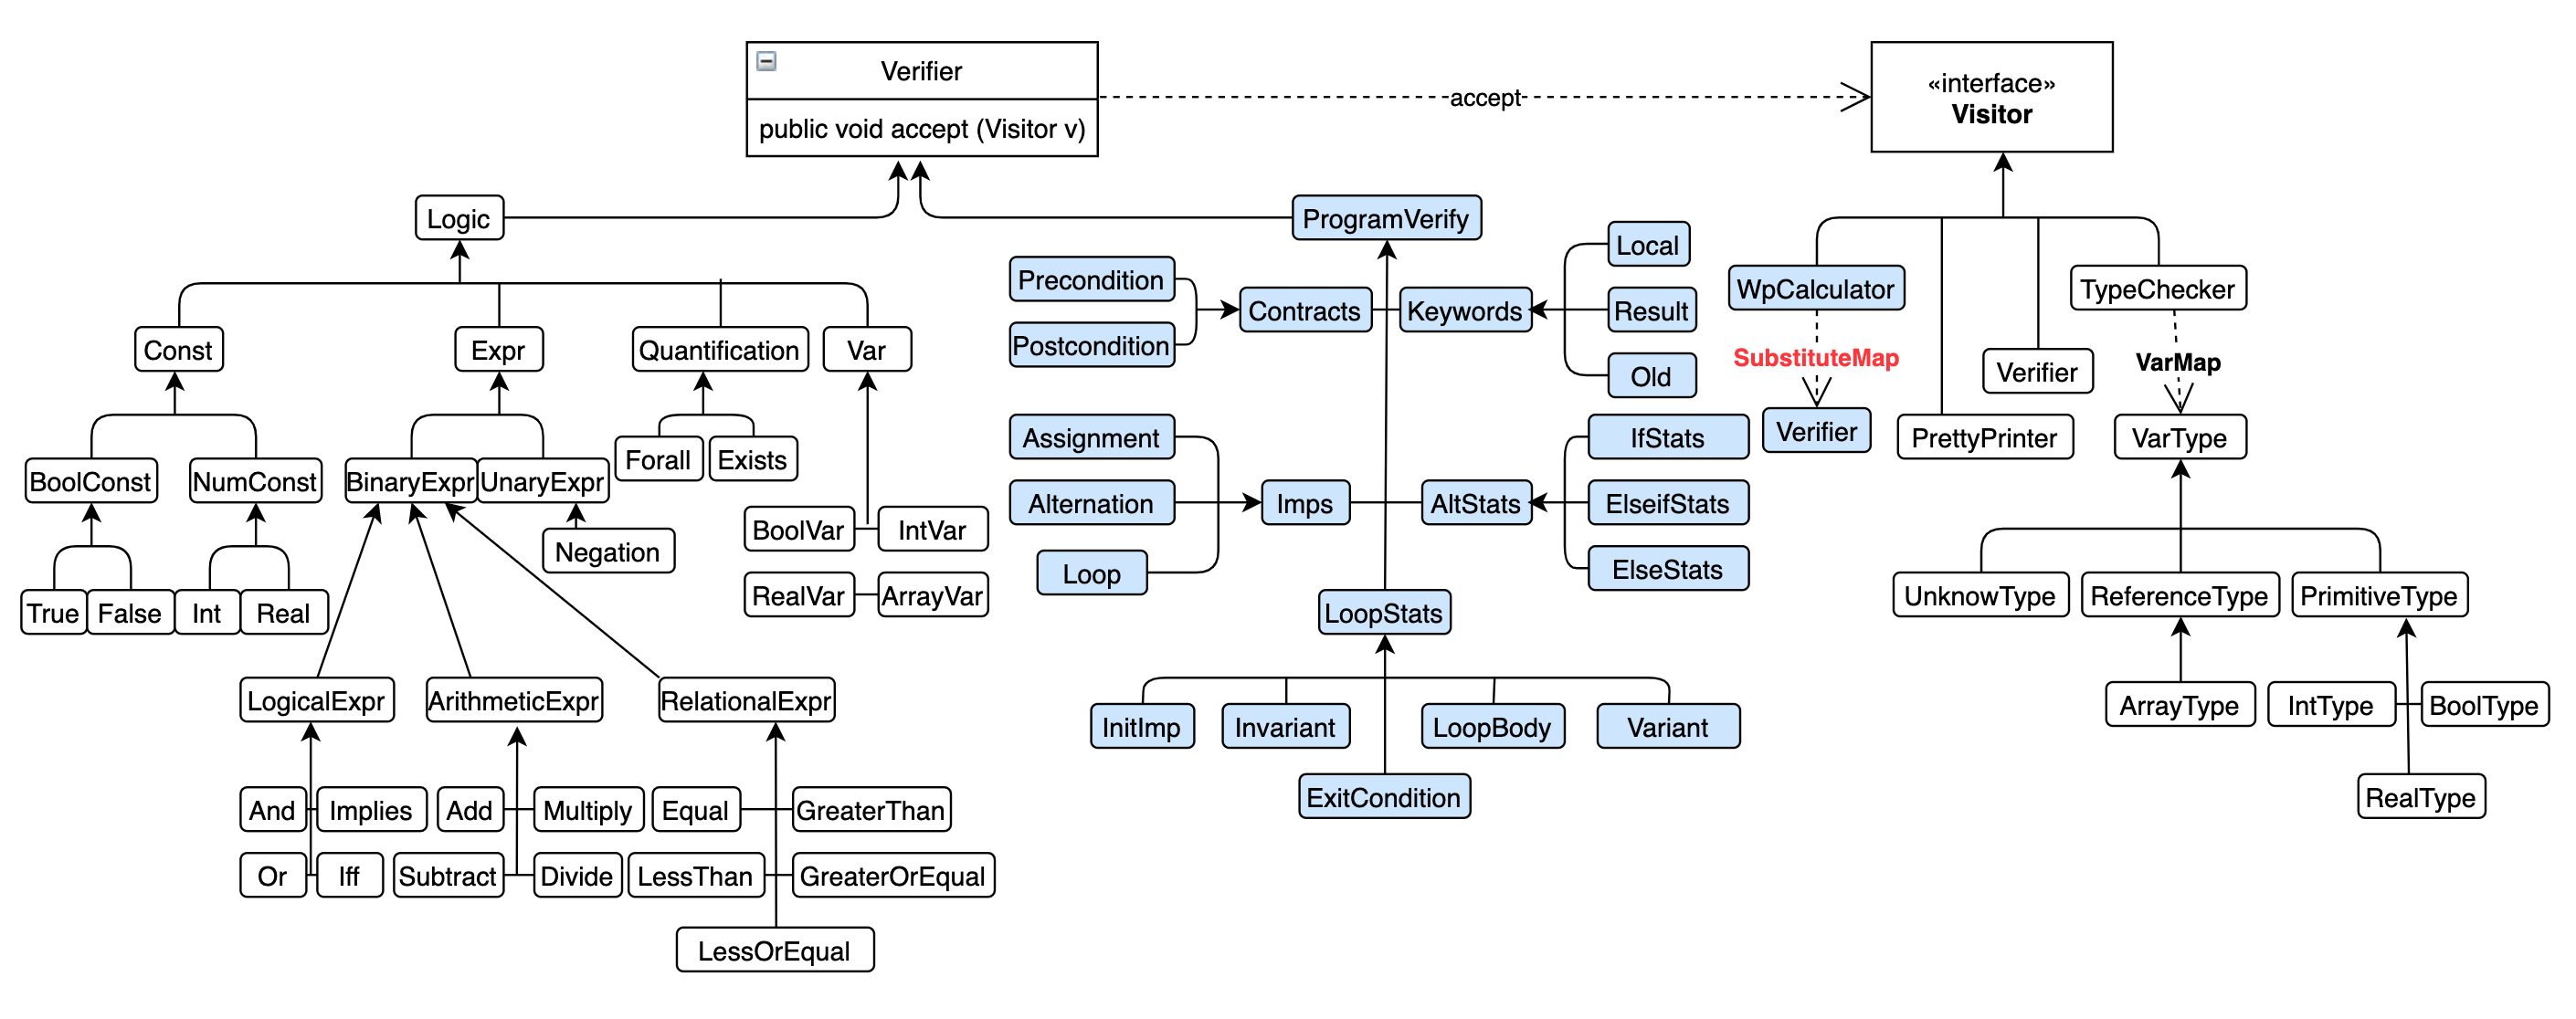
\includegraphics[width=\linewidth]{figures/Verifier_hiararchy}
% \captionof{figure}{\capcolor{Framework of Formalization and Verification}} 
\label{fig:framework}
\end{center}\graphspacing

\begin{enumerate} 
\item Specifying a contex-free grammar by using Antlr 4, supporting the input of propositions, predicates, and programs.
\item Parsing user input and generate the verifier objects. 
\item Apply the visitor design pattern to the verifier hierarchy for different purpose (e.g., type checking, pretty printing, wp calculating, etc.)
\item Send the generated output to the backend tool (i.e., Z3 SMT Solver) for verification.
\end{enumerate}


%%%%%%%%%%%%%%%%%%%%%%%%%%%%%%%%%%%%%%%%%%%%%%%%%%%%%%%%%%%%%%%%%%%%%%%%%%%%%%%%%%%%%%%%%%%%%%%%%%
%%%%%%%%%%%%%%%%%%%%%%%%%%%%%%%%%%%%% Hysteresis %%%%%%%%%%%%%%%%%%%%%%%%%%%%%%%%%%%%%%%%%%%%%%%%%
%%%%%%%%%%%%%%%%%%%%%%%%%%%%%%%%%%%%%%%%%%%%%%%%%%%%%%%%%%%%%%%%%%%%%%%%%%%%%%%%%%%%%%%%%%%%%%%%%%

{\color{Blue} \subsection*{Example of Propositional and Predicate Formula Verification}}
User input file:
\begin{lstlisting}
// Golden rule
p: BOOLEAN
q: BOOLEAN

// verify golden rule
verify (p and q <=> p) <=> (q <=> p or q)

// verify wrong version of golden rule
verify (p and q <=> p) <=> (q <=> p and q)
\end{lstlisting}
Program output:
\begin{lstlisting}
(((p and q) = p) = (q = (p or q)))
Is a tautology.

(((p and q) = p) = (q = (p and q)))
Where: 
    p : BOOLEAN
    q : BOOLEAN

Is not a tautology. Here is a counter example: 
    p : false
    q : true
\end{lstlisting}
\begin{itemize}
\item Example of formula verification: testing the Golden rule and its wrong version.
\item My Verifier will give the result if the formula is a tautology and provide counterexample otherwise.
\end{itemize}
%\noindent Based on the input-output declaration and ST implementation, as suppled by IEC~61131-3~\cite{IEC:2003:IEP}:
%
%% HYSTERESIS: declaration and ST implementation
%\begin{center}\graphspacing
%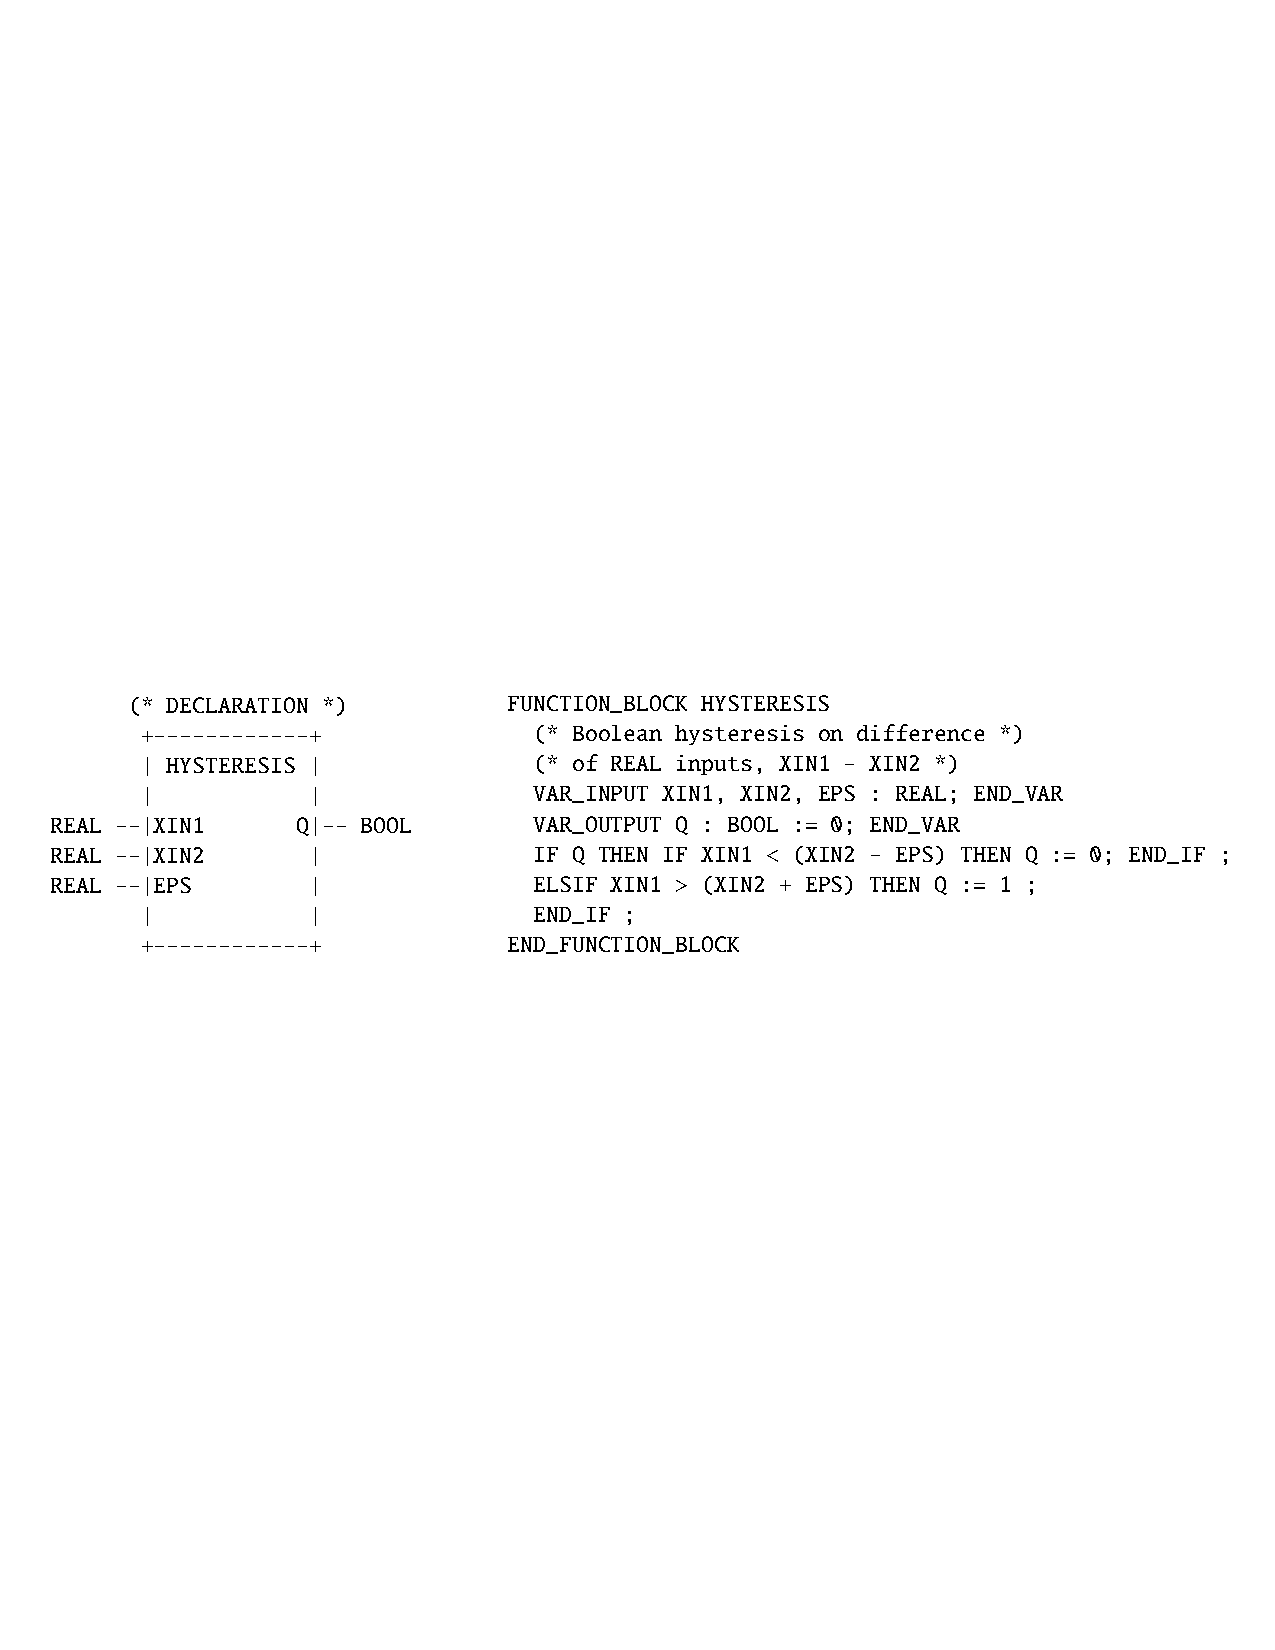
\includegraphics[width=\linewidth]{figures/hysteresis/hysteresis_decl}
%% \captionof{figure}{\capcolor{Hysteresis: Declaration and ST Implementation~\cite{IEC:2003:IEP}}}
%\end{center}\graphspacing
%
%\noindent We derive the tabular requirement for \var{HYSTERESIS}:
%
%% HYSTERESIS: expected behaviour in tabular expression 
%\begin{center}\graphspacing
%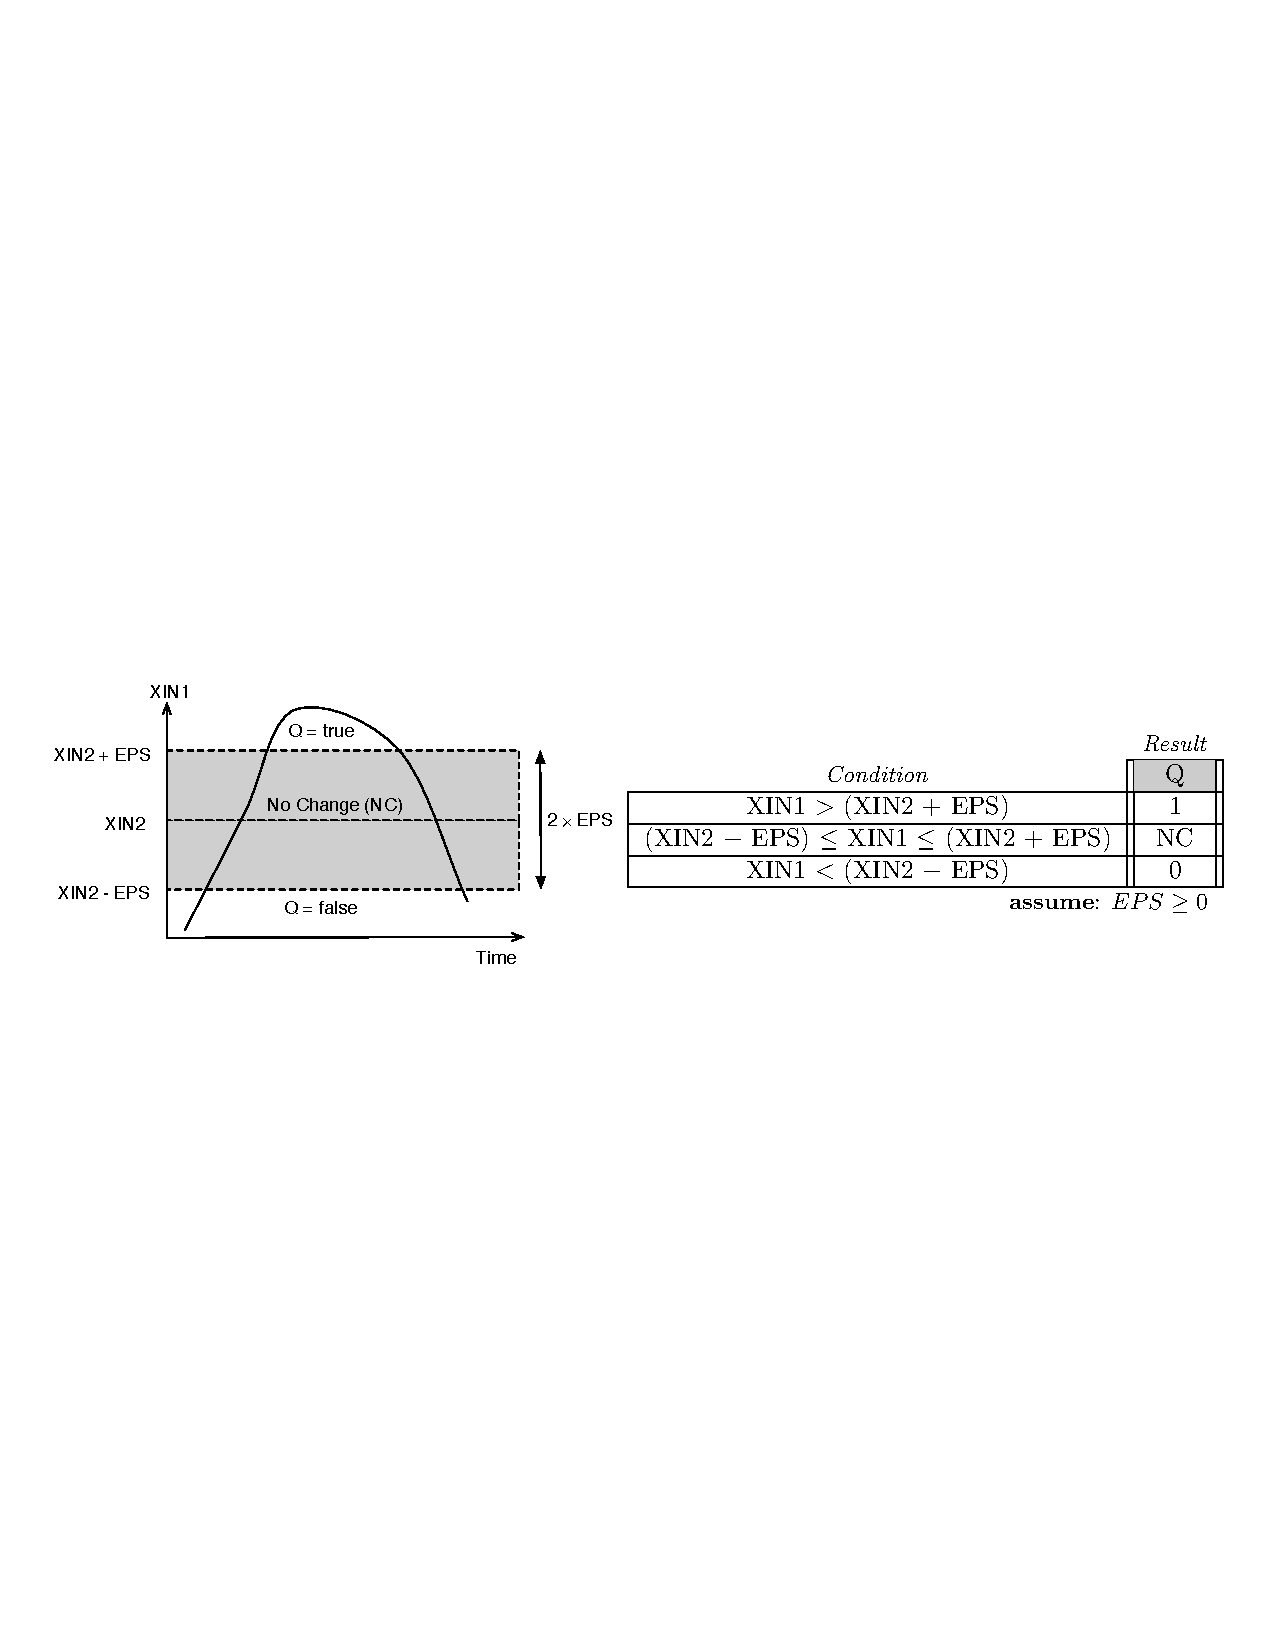
\includegraphics[width=\linewidth]{figures/hysteresis/hysteresis_tab_req}
%% \captionof{figure}{\capcolor{Hysteresis: Expected Behaviour \& Tabular Requirement}}
%\end{center}\graphspacing
%
%\noindent To prove that the ST implementation of \var{HYSTERESIS}, supplied by IEC~61131-3, satisfies its tabular requirements, we formalize it in PVS:
%
%% HYSTERESIS: ST implementation in pvs
%\begin{center}\graphspacing
%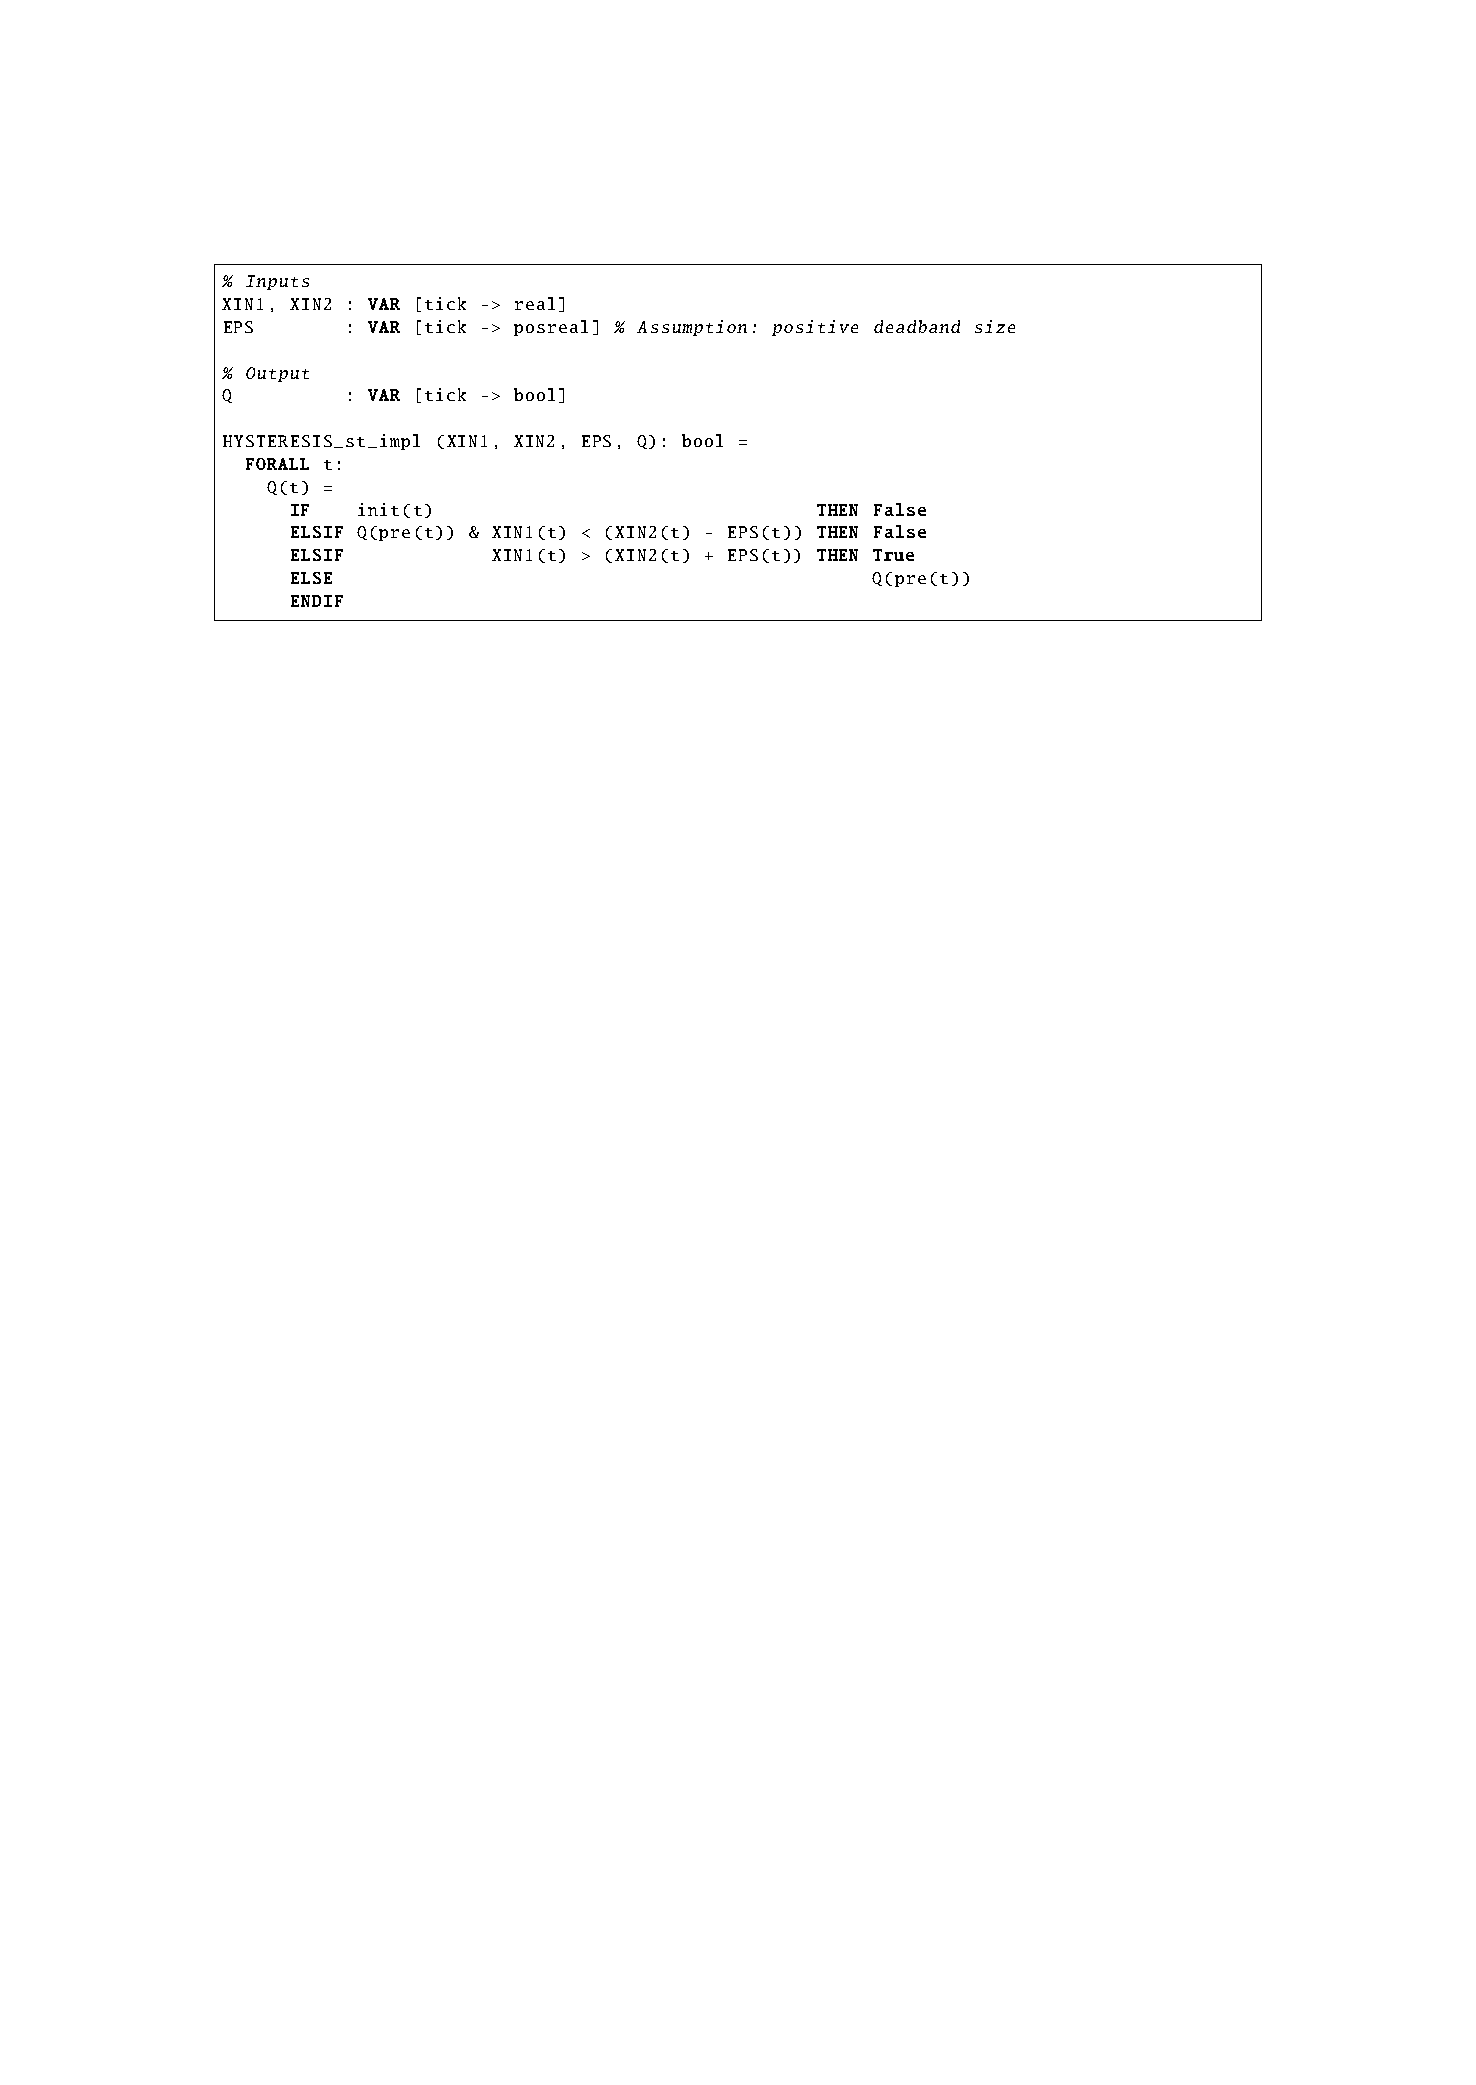
\includegraphics[width=\linewidth]{figures/hysteresis/hysteresis_pvs_st_impl}
%% \captionof{figure}{\capcolor{Hysteresis: ST Implementation in PVS}}
%\end{center}\graphspacing
%
%\noindent We also translate the tabular requirement of \var{HYSTERESIS} into PVS:
%
%% HYSTERESIS: tabular requirement in pvs
%\begin{center}\graphspacing
%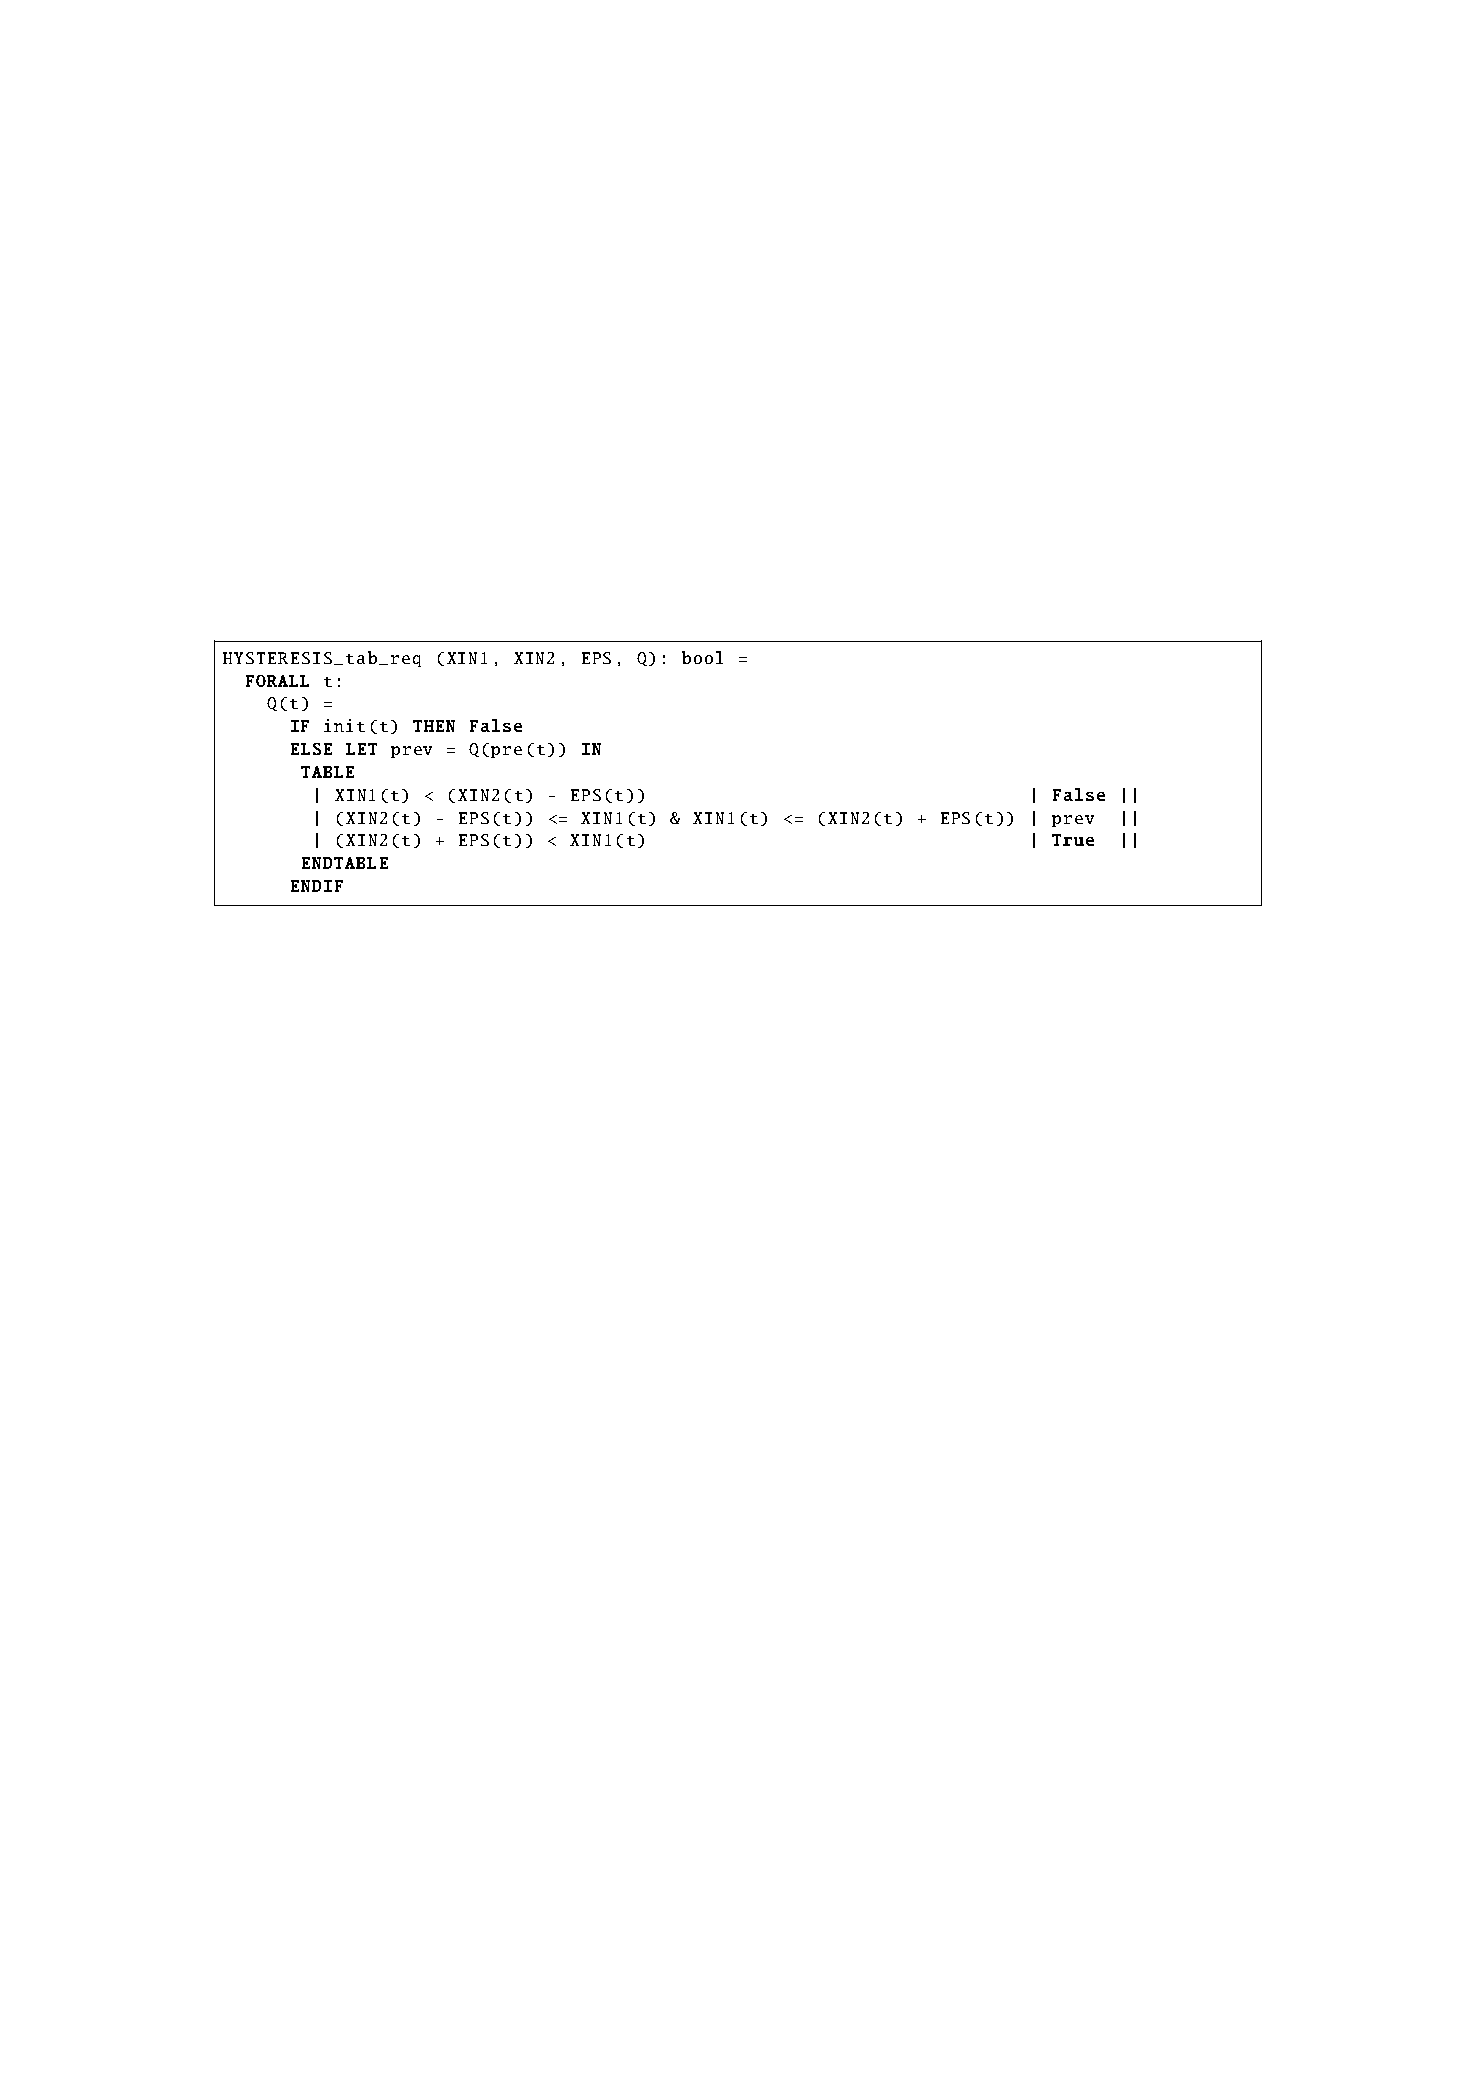
\includegraphics[width=\linewidth]{figures/hysteresis/hysteresis_pvs_tab_req}
%% \captionof{figure}{\capcolor{Hysteresis: Tabular Requirement in PVS}}
%\end{center}\graphspacing
%
%\noindent Finally, we prove that the ST implementation is:
%\begin{itemize}
%\item {\color{BrickRed} \emph{correct}} (i.e..,~satisfies its requirement)
%\item {\color{BrickRed} \emph{consistent}} (i.e.,~each input vector has a corresponding output)
%\end{itemize}
%
%% HYSTERESIS: proofs of correctness and consistency in pvs
%\begin{center}\graphspacing
%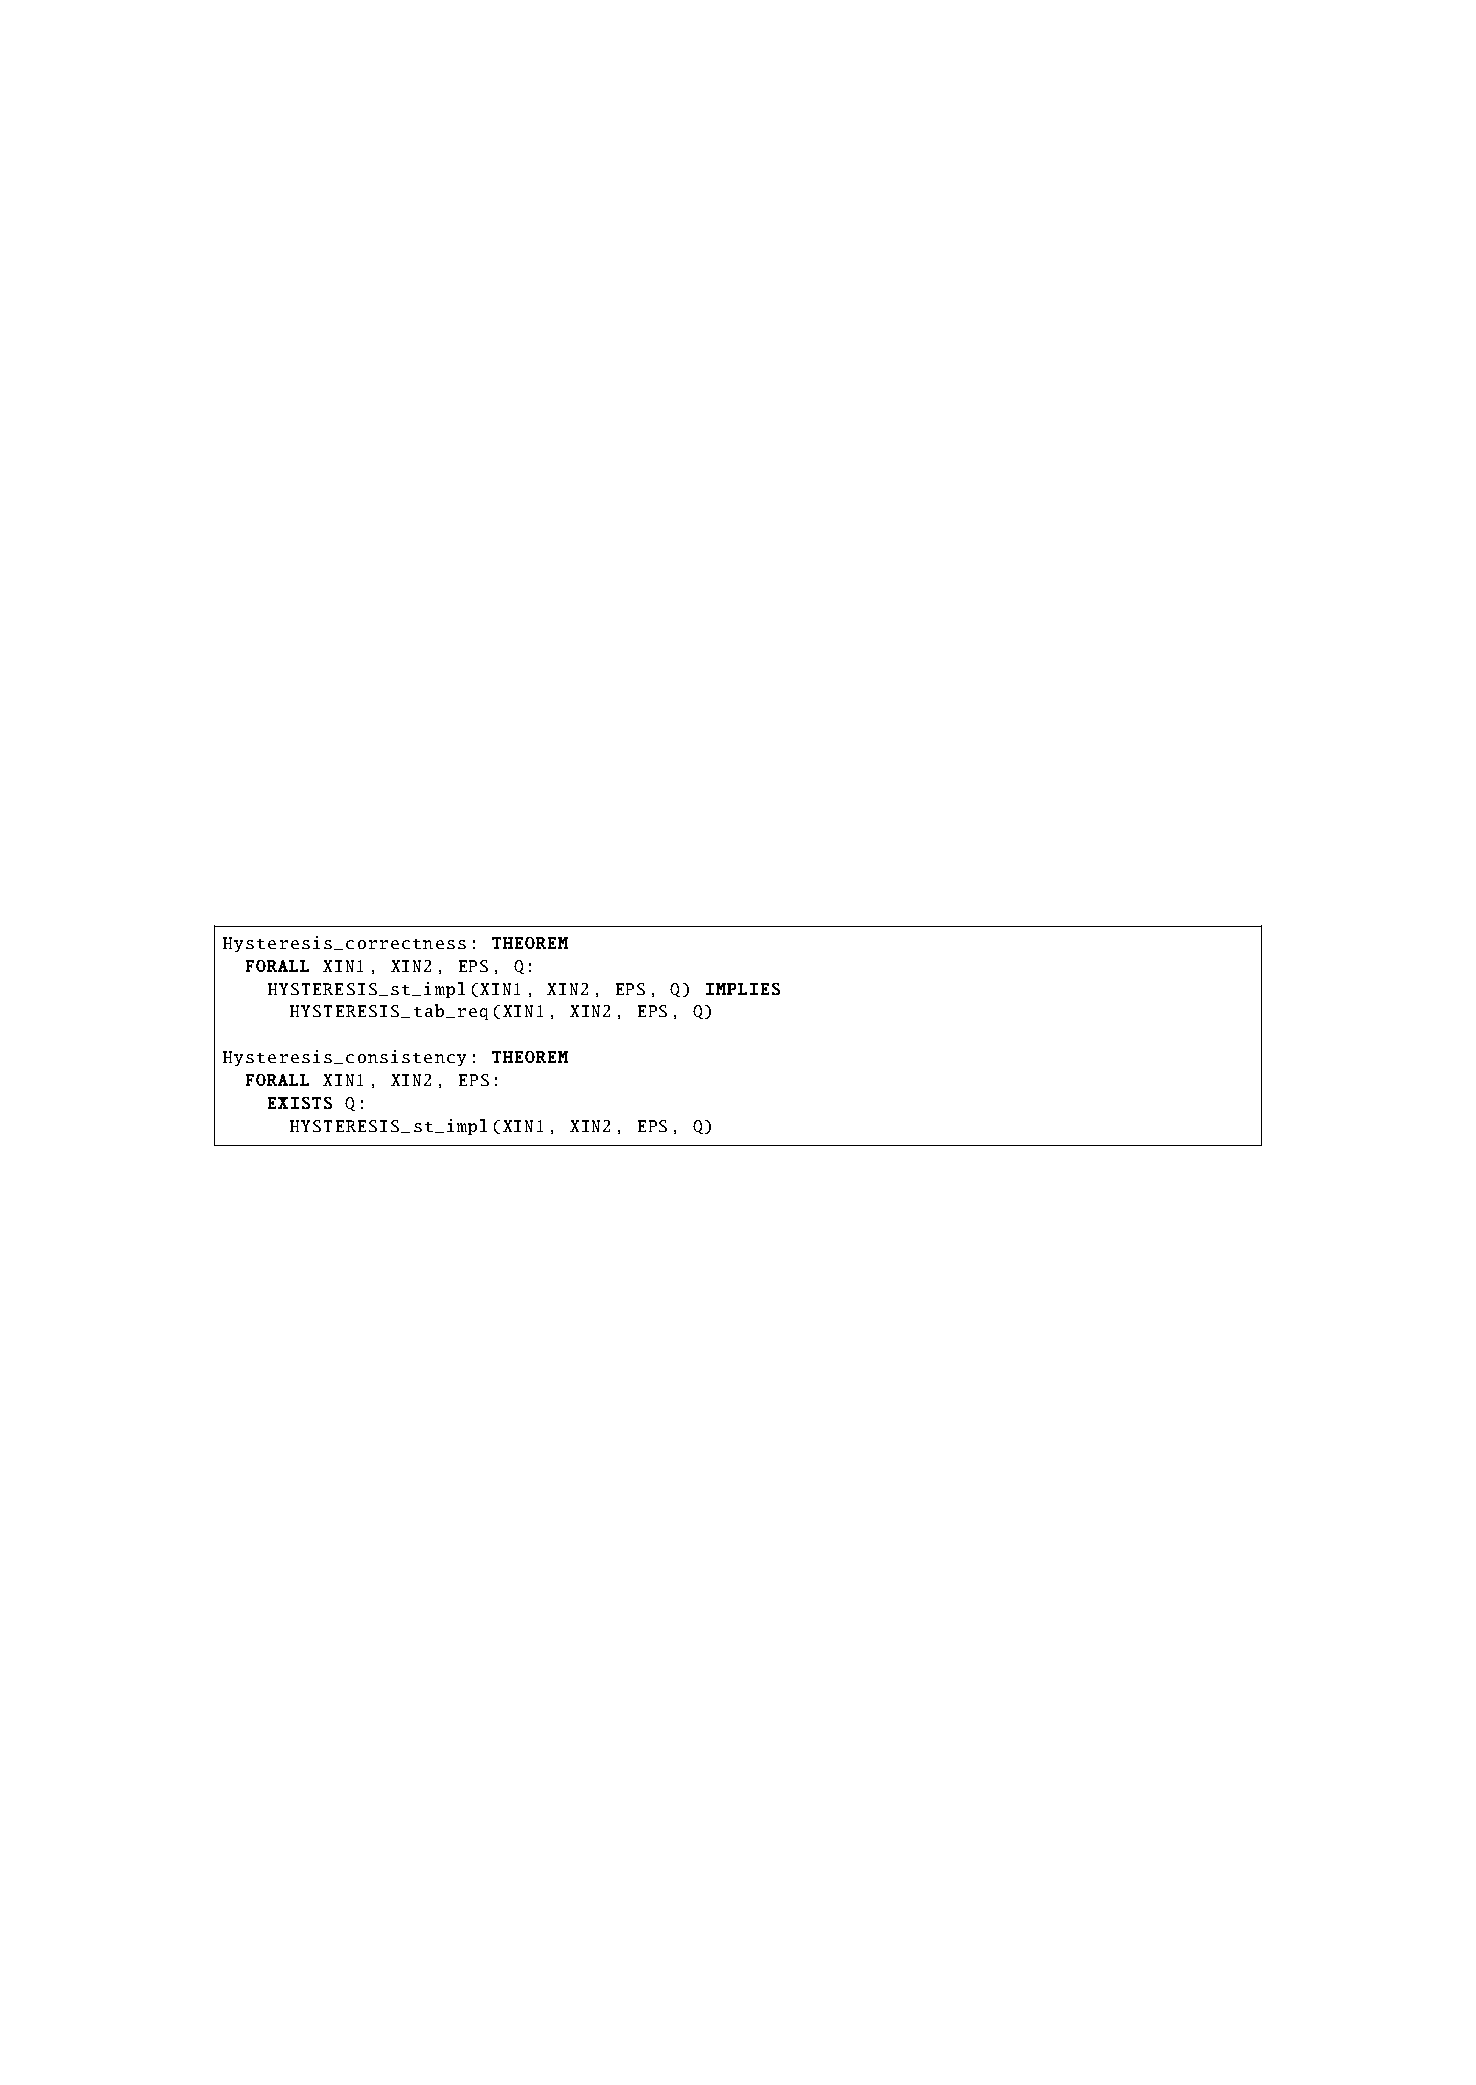
\includegraphics[width=\linewidth]{figures/hysteresis/hysteresis_pvs_theorems}
%% \captionof{figure}{\color{Red} Hysteresis: Correctness and Consistency Theorems in PVS}
%\end{center}\graphspacing
%
%\noindent \textbf{Remark}. Upon certifying the \var{HYSTERESIS} block, we may reuse its requirements predicate \var{HYSTERESIS\_tab\_req} to certify others (e.g., the \var{LIMITS\_ALARM} block) that use it as a component. 

%%%%%%%%%%%%%%%%%%%%%%%%%%%%%%%%%%%%%%%%%%%%%%%%%%%%%%%%%%%%%%%%%%%%%%%%%%%%%%%%%%%%%%%%%%%%%%%%%%
%%%%%%%%%%%%%%%%%%%%%%%%%%%%%%%%%%%%% Limits Alarm %%%%%%%%%%%%%%%%%%%%%%%%%%%%%%%%%%%%%%%%%%%%%%%
%%%%%%%%%%%%%%%%%%%%%%%%%%%%%%%%%%%%%%%%%%%%%%%%%%%%%%%%%%%%%%%%%%%%%%%%%%%%%%%%%%%%%%%%%%%%%%%%%%

{\color{Blue} \subsection*{Example of Program Verification (1)}}
User input file:
\begin{lstlisting}
-- Change the value of array at index i

change_at(a:ARRAY[REAL]; i : INTEGER; nv: REAL)
require
	valid_index: a.lower <= i and i <= a.upper
local
	x: INTEGER
	y: BOOLEAN
do
	a[i] := nv;
ensure
	changed: a[i] = nv
	unchanged: forall j:INTEGER; |(a.lower <= j and j <= a.upper and not i = j) => old a[j] = a[j]
	test_wrong_postcondition: not a[i] = nv
end

verify change_at
\end{lstlisting}
Program output:
\begin{lstlisting}
change_at(a : ARRAY[REAL];i : INTEGER;nv : REAL)
  local
    x : INTEGER
    y : BOOLEAN
  require
    valid_index : ((a.lower <= i) and (i <= a.upper))
  do
    a[i] := nv;
  ensure
    changed : (a[i] = nv)
    unchanged : forall j | ((((a.lower <= j) and (j <= a.upper)) and (not (i = j))) => (old a[j] = a[j]))
    test_wrong_postcondition : (not (a[i] = nv))
  end

Where: 
Precondition(Q) : 
    valid_index : ((a.lower <= i) and (i <= a.upper))
Postcondition(R) : 
    changed : (a[i] = nv)
    unchanged : forall j | ((((a.lower <= j) and (j <= a.upper)) and (not (i = j))) => (old a[j] = a[j]))
    test_wrong_postcondition : (not (a[i] = nv))
Implementation(S) : 
    a[i] := nv;

wp(S, changed)
  (nv = nv)
wp(S, unchanged)
  forall j | ((((a.lower <= j) and (j <= a.upper)) and (not (i = j))) => (old a[j] = a[j]))
wp(S, test_wrong_postcondition)
  (not (nv = nv))

Proof Obligation: 
(valid_index) => wp(S, changed)
Discharged.
(valid_index) => wp(S, unchanged)
Discharged.
(valid_index) => wp(S, test_wrong_postcondition)
Not discharged.
Counterexample is not available.
\end{lstlisting}
\begin{itemize}
\item My Verifier supports the {\bf Old} keyword.
\item My Verifier provides the detail of program specification and weakest postcondition (wp).
\item My Verifier requires user to specify the tag for each precondition and postcondition, for the result of verification, my Verifier will indicates the status of wp for each postcondition (e.g., discharged / not discharged). User of my Verifier could easily locate which postcondition is violated.
\end{itemize}

{\color{Blue} \subsection*{Example of Program Verification (2)}}
User input file:
\begin{lstlisting}
-- Find the maximum element in array a and return it

find_max (a: ARRAY[INTEGER]) : INTEGER
require
	no_restriction: a.count > 0
local
	i: INTEGER
do
	from
		i := a.lower;
		Result := a[i];
	invariant
		loop_invariant: forall j: INTEGER; | (a.lower <= j and j < i) => (Result >= a[j])
	until
		i > a.upper
	loop
		if a[i] > Result then
			Result := a[i];
		end
		i := i + 1;
	variant
		loop_variant: a.upper - i + 1
	end
ensure
	correct_result: forall k: INTEGER; | (a.lower <= k and k <= a.upper) => (Result >= a[k])
	not_changed: forall s:INTEGER; | (a.lower <= s and s <= a.upper) => (a[s] = old a[s])
end

verify find_max
\end{lstlisting}
Program output:
\begin{lstlisting}
find_max(a : ARRAY[INTEGER]) : INTEGER
  local
    i : INTEGER
  require
    no_restriction : (a.count > 0)
  do
from
    i := a.lower;
    Result := a[i];
invariant
  loop_invariant : forall j | (((a.lower <= j) and (j < i)) => (Result >= a[j]))
until
  (i > a.upper)
loop
    if (a[i] > Result) then
      Result := a[i];
    end
    i := (i + 1);
variant
  loop_variant : ((a.upper - i) + 1)
end
  ensure
    correct_result : forall k | (((a.lower <= k) and (k <= a.upper)) => (Result >= a[k]))
    not_changed : forall s | (((a.lower <= s) and (s <= a.upper)) => (a[s] = old a[s]))
  end

Where: 
Precondition(Q) : 
    no_restriction : (a.count > 0)
Postcondition(R) : 
    correct_result : forall k | (((a.lower <= k) and (k <= a.upper)) => (Result >= a[k]))
    not_changed : forall s | (((a.lower <= s) and (s <= a.upper)) => (a[s] = old a[s]))
Implementation(S) : 
from
    i := a.lower;
    Result := a[i];
invariant
  loop_invariant : forall j | (((a.lower <= j) and (j < i)) => (Result >= a[j]))
until
  (i > a.upper)
loop
    if (a[i] > Result) then
      Result := a[i];
    end
    i := (i + 1);
variant
  loop_variant : ((a.upper - i) + 1)
end
Correctness conditions : 
1. Given precondition Q, the initialization step Sinit establishes LI I : {Q} Sinit {I}
  ((a.count > 0) => forall j | (((a.lower <= j) and (j < a.lower)) => (a[a.lower] >= a[j])))

2. At the end of Sbody, if not yet to exit, LI I is maintained : {I and (not B)} Sbody {I}
  ((forall j | (((a.lower <= j) and (j < i)) => (Result >= a[j])) and (not (i > a.upper))) => (((a[i] > Result) => forall j | (((a.lower <= j) and (j < (i + 1))) => (a[i] >= a[j]))) and ((not (a[i] > Result)) => forall j | (((a.lower <= j) and (j < (i + 1))) => (Result >= a[j])))))

3. If ready to exit and LI I maintained, postcondition R is established : I and B => R

  3-1. I and B => correct_result : ((forall j | (((a.lower <= j) and (j < i)) => (Result >= a[j])) and (i > a.upper)) => forall k | (((a.lower <= k) and (k <= a.upper)) => (Result >= a[k])))

  3-2. I and B => not_changed : ((forall j | (((a.lower <= j) and (j < i)) => (Result >= a[j])) and (i > a.upper)) => forall s | (((a.lower <= s) and (s <= a.upper)) => (a[s] = old a[s])))

4. Given LI I, and not yet to exit, Sbody maintains LV V as non-negative : {I and (not B)} Sbody {V >= 0}
  ((forall j | (((a.lower <= j) and (j < i)) => (Result >= a[j])) and (not (i > a.upper))) => (((a[i] > Result) => (((a.upper - (i + 1)) + 1) >= 0)) and ((not (a[i] > Result)) => (((a.upper - (i + 1)) + 1) >= 0))))

5. Given LI I, and not yet to exit, Sbody decrements LV V : {I and (not B)} Sbody {V < V0}
  ((forall j | (((a.lower <= j) and (j < i)) => (Result >= a[j])) and (not (i > a.upper))) => (((a[i] > Result) => (((a.upper - (i + 1)) + 1) < ((a.upper - i) + 1))) and ((not (a[i] > Result)) => (((a.upper - (i + 1)) + 1) < ((a.upper - i) + 1)))))

Condition 1 is discharged.
Condition 2 is discharged.
Condition 3 postcondition correct_result is discharged.
Condition 3 postcondition not_changed is discharged.
Condition 4 is discharged.
Condition 5 is discharged.
\end{lstlisting}
\begin{itemize}
\item My Verifier supports the {\bf Result} keyword.
\item For programs that contains the loop, my Verifier will follow the wp calculation rule and provide the result and status of the five conditions.
\end{itemize}
%\noindent Based on the input-output declaration and FBD implementation, as suppled by IEC~61131-3~\cite{IEC:2003:IEP}:
%
%% LIMITS_ALARM: declaration and FBD implementation
%\begin{center}\graphspacing
%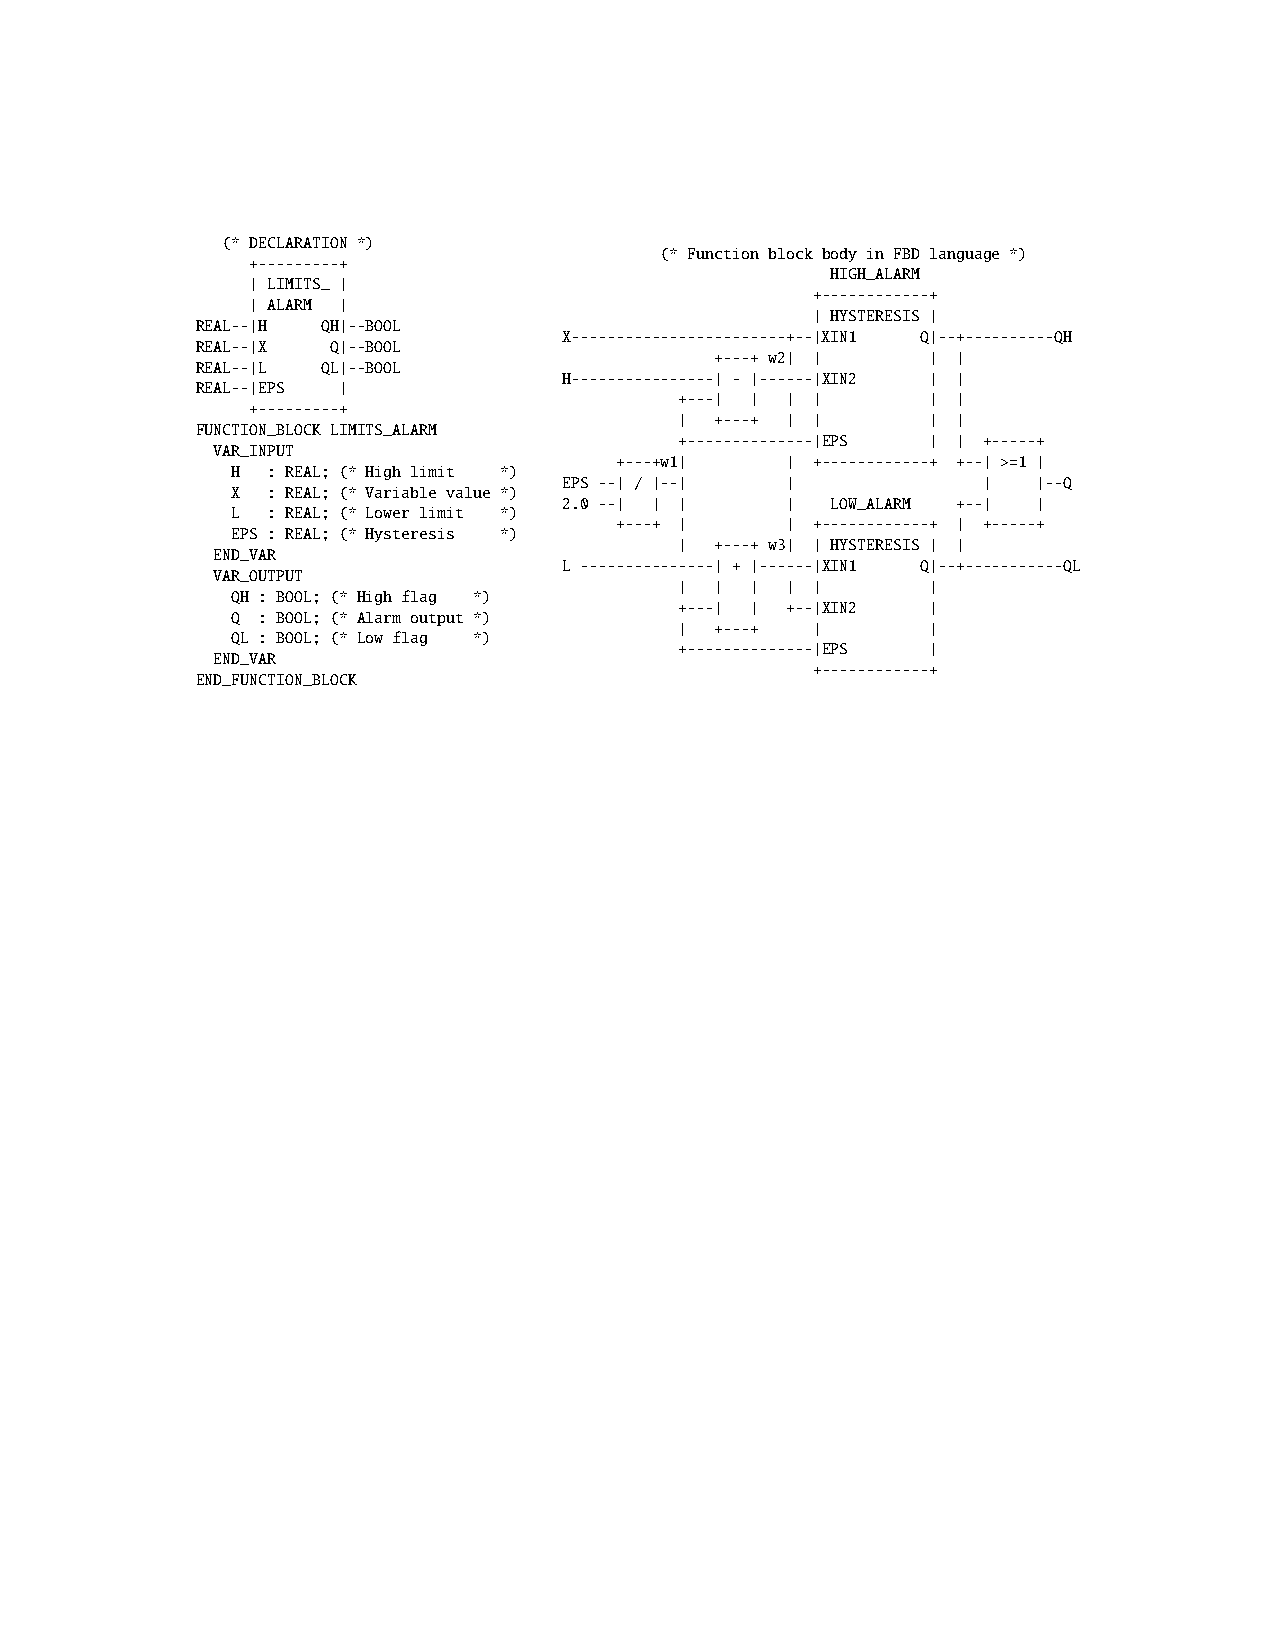
\includegraphics[width=\linewidth]{figures/limits_alarm/limits_alarm_decl}
%% \captionof{figure}{\capcolor{Limits Alarm: Declaration and FBD Implementation~\cite{IEC:2003:IEP}}}
%\end{center}\graphspacing
%
%\noindent We derive the tabular requirement for \var{LIMITS\_ALARM}:
%
%% LIMITS_ALARM: expected behaviour in tabular expression 
%\begin{center}\graphspacing
%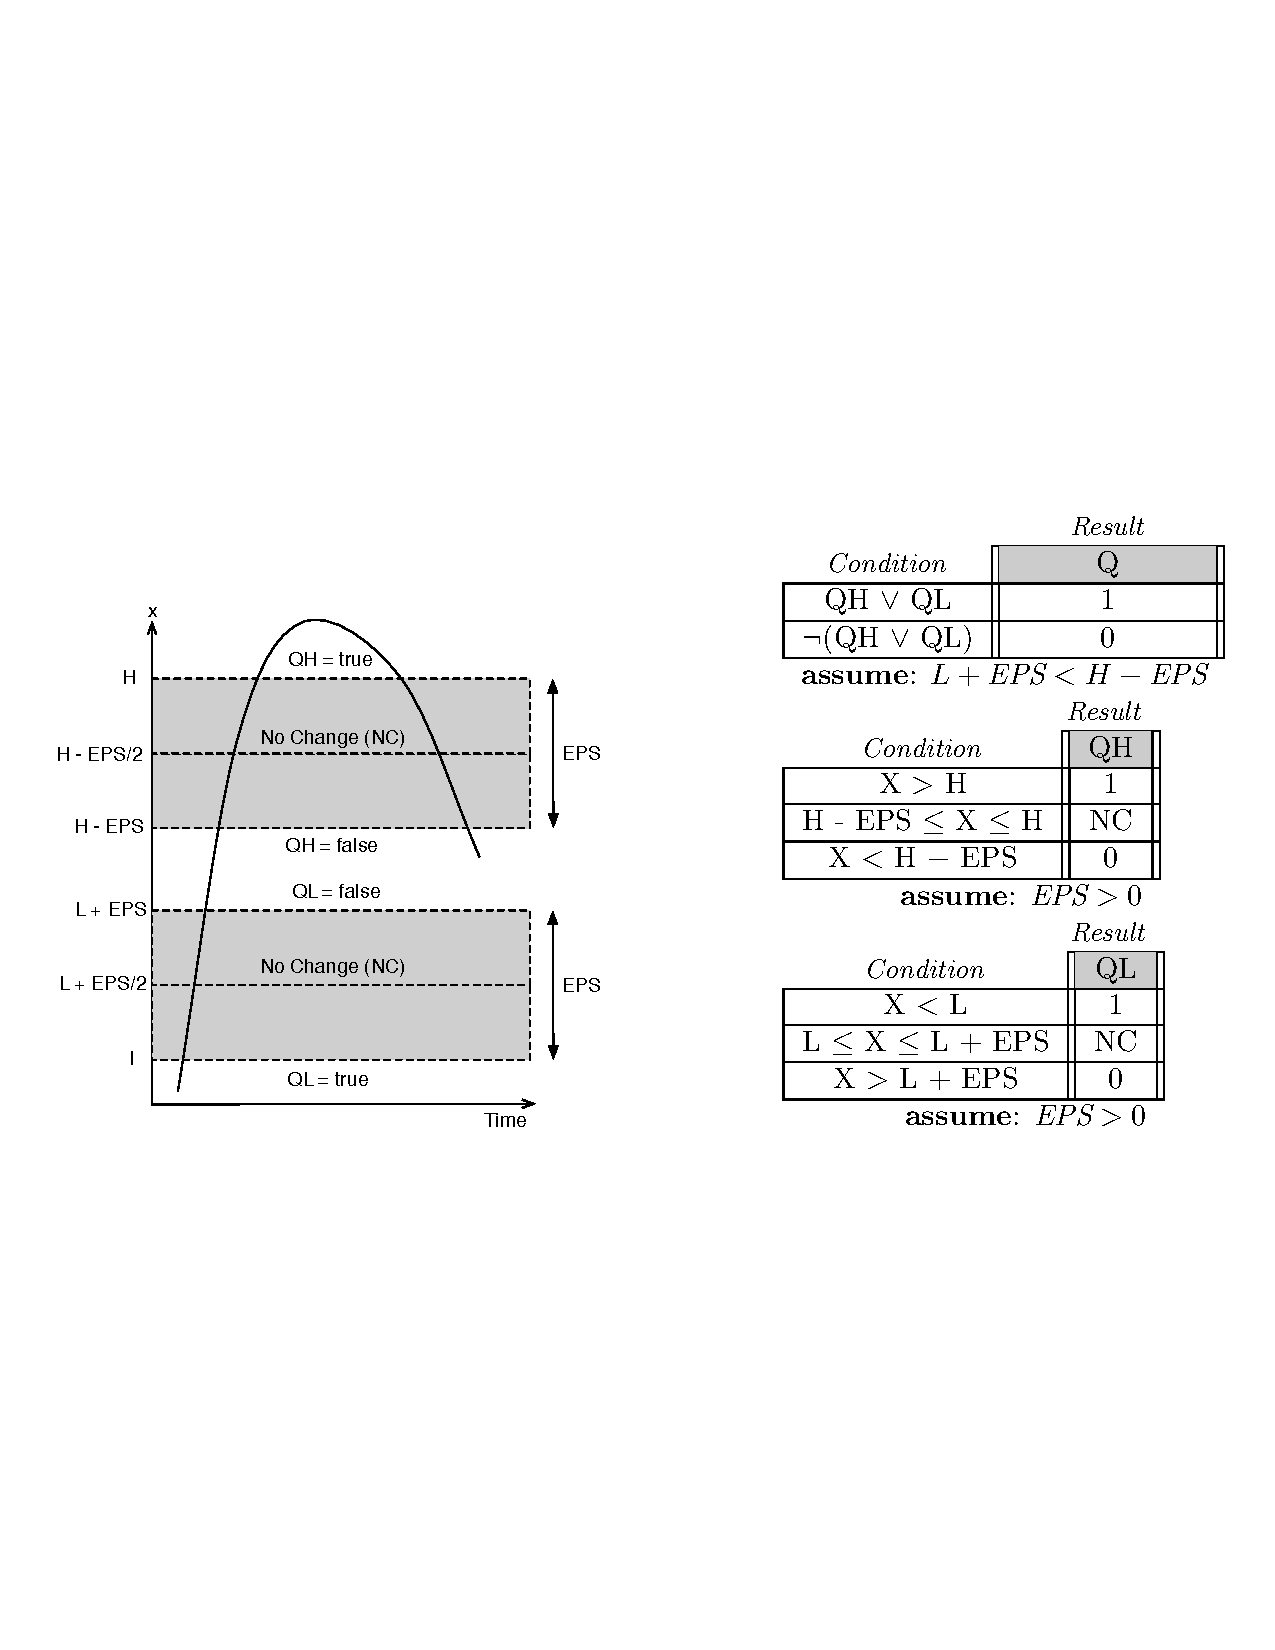
\includegraphics[width=\linewidth]{figures/limits_alarm/limits_alarm_tab_req}
%% \captionof{figure}{\capcolor{Limits Alarm: Expected Behaviour \& Tabular Requirements}}
%\end{center}\graphspacing
%
%\noindent We formalize the FBD implementation of \var{LIMITS\_ALARM} and its tabular requirements in PVS:
%
%% LIMITS_ALARM: FBD implementation in pvs
%\begin{center}\graphspacing
%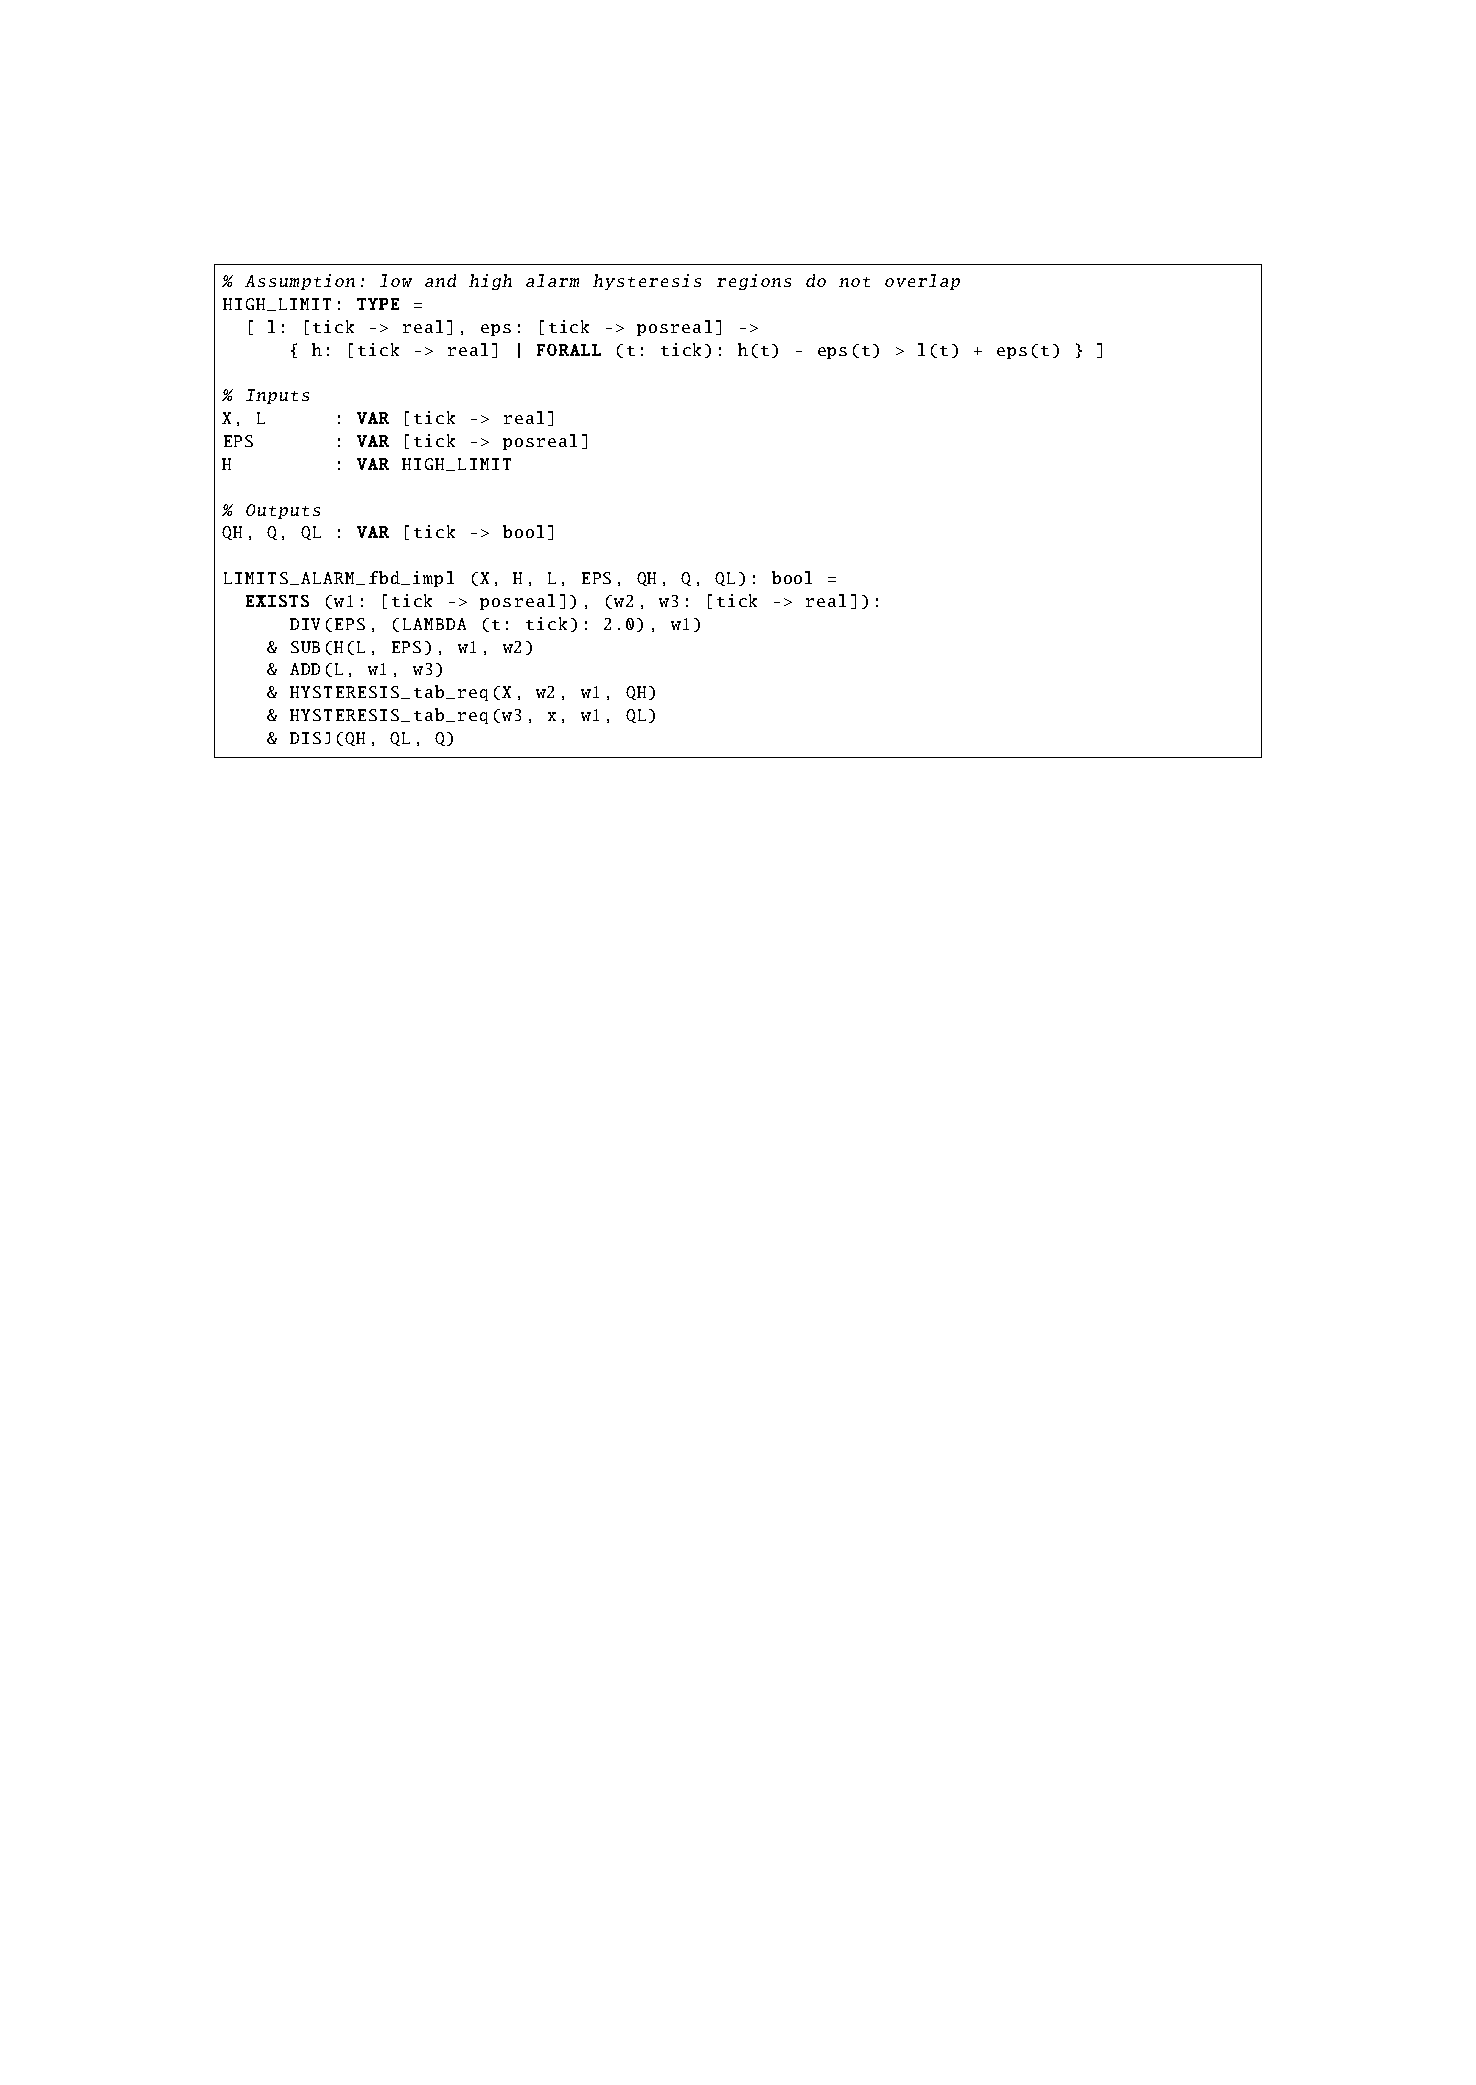
\includegraphics[width=\linewidth]{figures/limits_alarm/limits_alarm_pvs_fbd_impl}
%% \captionof{figure}{\capcolor{Limits Alarm: FBD Implementation in PVS}}
%\end{center}\graphspacing
%
%\noindent Finally, we prove that the FBD implementation of \var{LIMITS\_ALARM} is {\color{BrickRed} \emph{correct}} and {\color{BrickRed} \emph{consistent}}.
%
%% LIMITS_ALARM: correctness and consistency 
%\begin{center}\graphspacing
%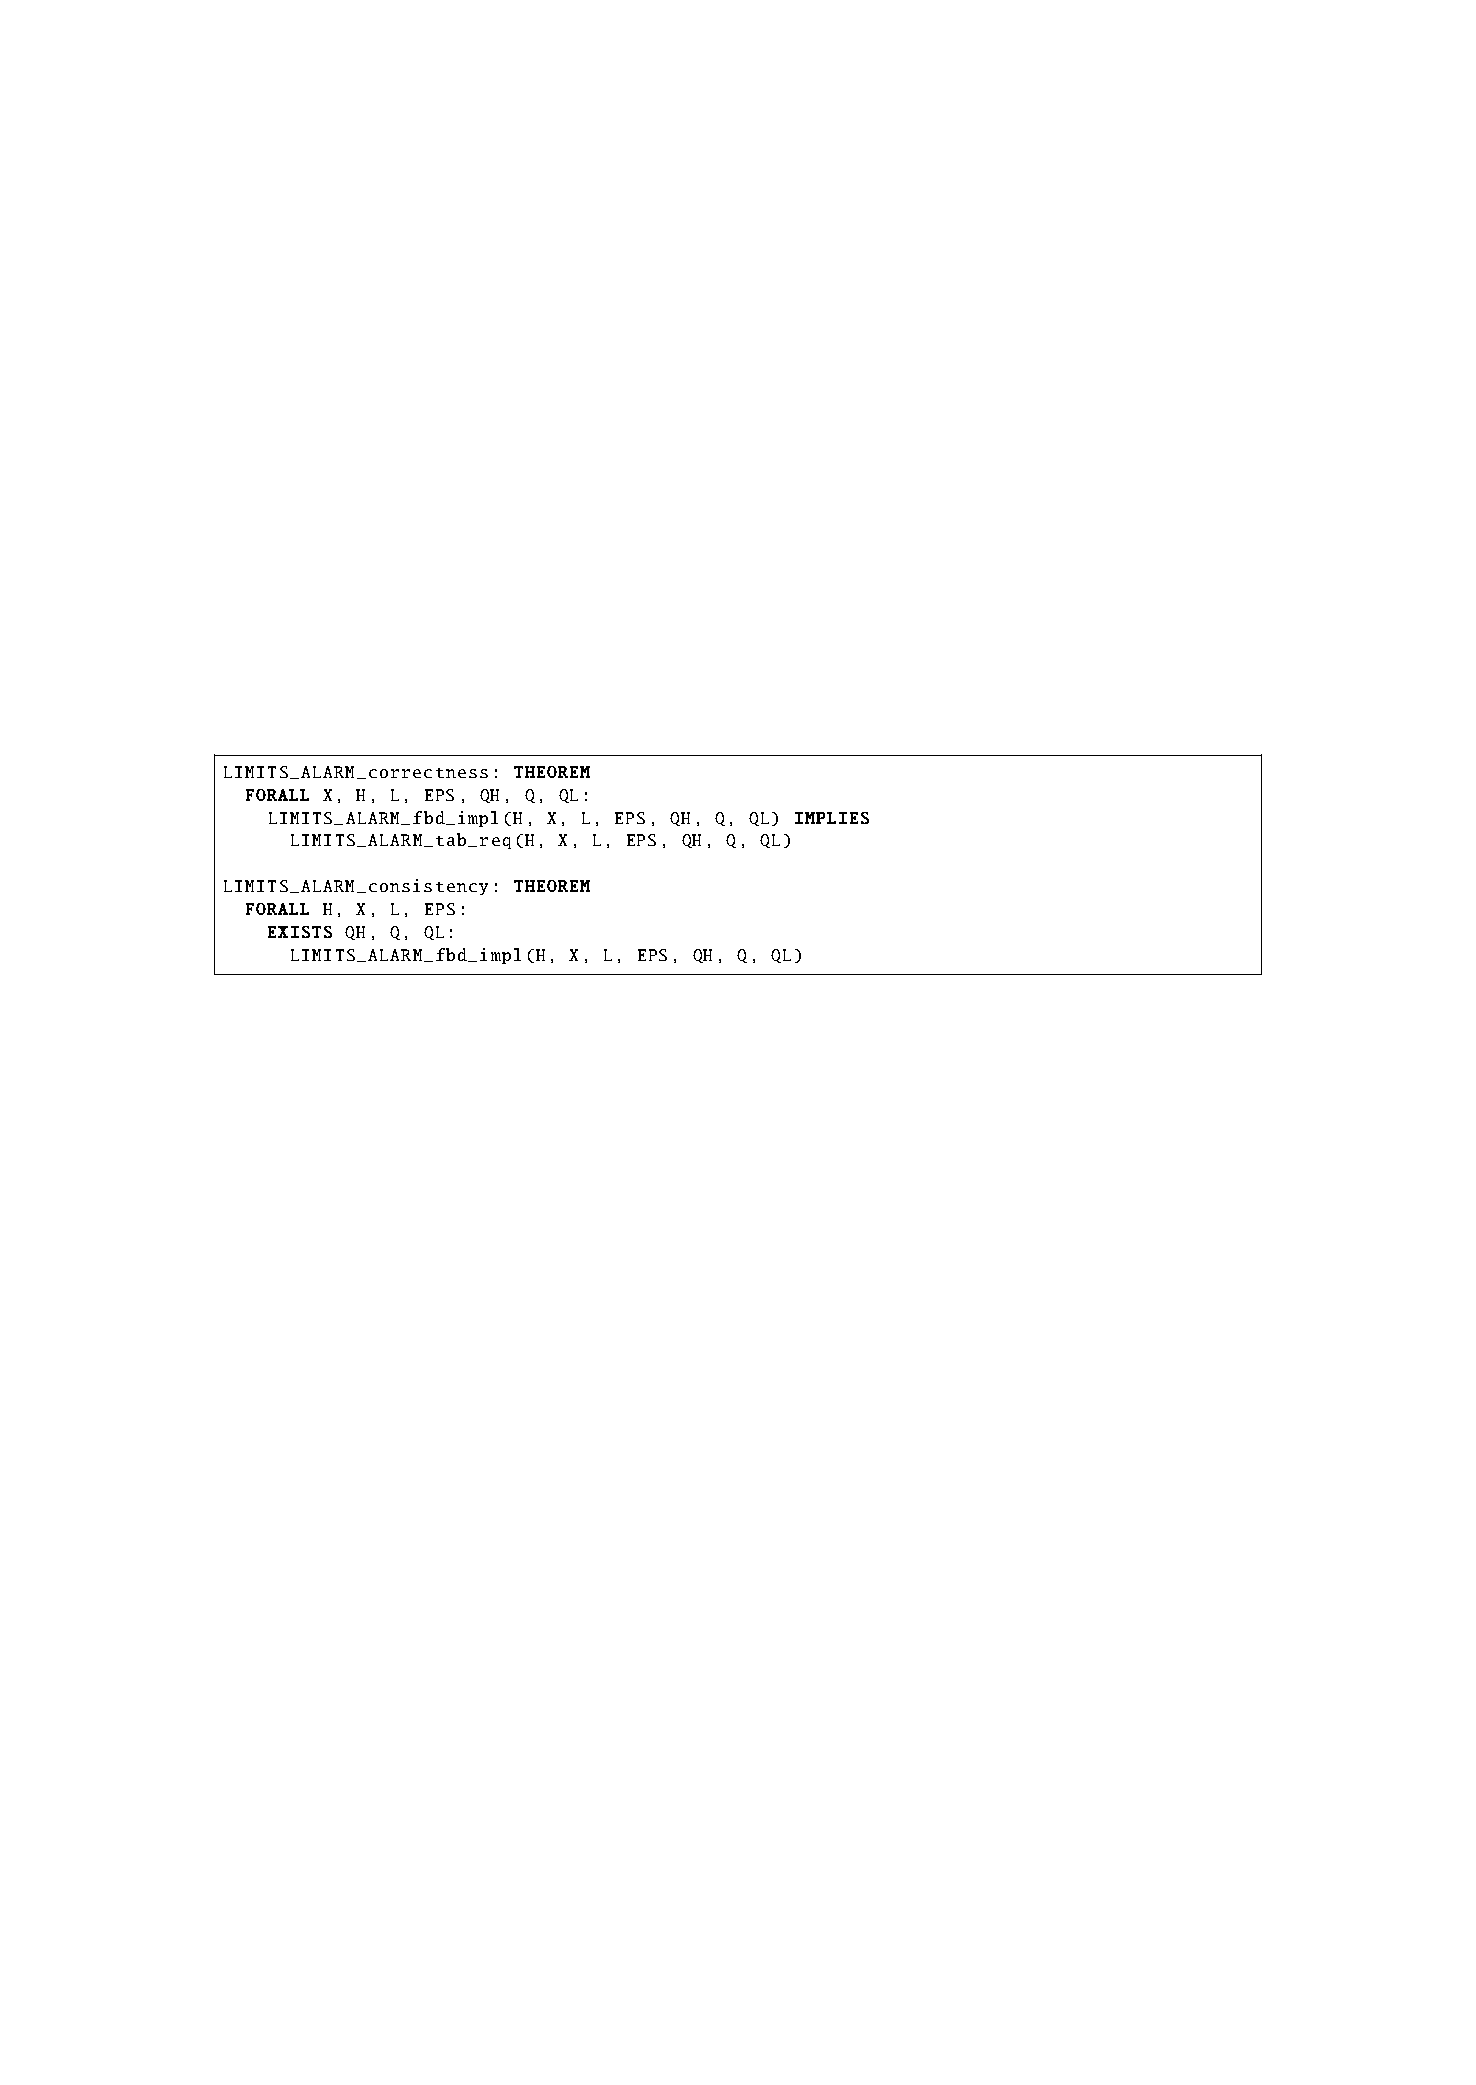
\includegraphics[width=\linewidth]{figures/limits_alarm/limits_alarm_pvs_theorems}
%% \captionof{figure}{\color{Red} Limits Alarm: Correctness and Consistency Theorems in PVS}
%\end{center}\graphspacing

%%%%%%%%%%%%%%%%%%%%%%%%%%%%%%%%%%%%%%%%%%%%%%%%%%%%%%%%%%%%%%%%%%%%%%%%%%%%%%%%%%%%%%%%%%%%%%%%%%
%%%%%%%%%%%%%%%%%%%%%%%%%%%%%%%%%%%%% Future Work %%%%%%%%%%%%%%%%%%%%%%%%%%%%%%%%%%%%%%%%%%%%%%%%
%%%%%%%%%%%%%%%%%%%%%%%%%%%%%%%%%%%%%%%%%%%%%%%%%%%%%%%%%%%%%%%%%%%%%%%%%%%%%%%%%%%%%%%%%%%%%%%%%%

{\color{Blue} \subsection*{Forthcoming Research}}
\begin{itemize}
	\item Verification of the computer program that contains nested loop and recursive methods.
	\item Providing counterexample for array and quantifications.
\end{itemize}
%%%%%%%%%%%%%%%%%%%%%%%%%%%%%%%%%%%%%%%%%%%%%%%%%%%%%%%%%%%%%%%%%%%%%%%%%%%%%%%%%%%%%%%%%%%%%%%%%%
%%%%%%%%%%%%%%%%%%%%%%%%%%%%%%%%%%%%% References %%%%%%%%%%%%%%%%%%%%%%%%%%%%%%%%%%%%%%%%%%%%%%%%%
%%%%%%%%%%%%%%%%%%%%%%%%%%%%%%%%%%%%%%%%%%%%%%%%%%%%%%%%%%%%%%%%%%%%%%%%%%%%%%%%%%%%%%%%%%%%%%%%%%

\nocite{*} % Print all references regardless of whether they were cited in the poster or not
\renewcommand{\refname}{{\normalsize \color{Blue} References}}
{\small
\bibliographystyle{plain}
\bibliography{fbs_poster_refs}} 

\end{multicols}
\end{document}